\documentclass[master, och, diploma]{SCWorks}
% Тип обучения (одно из значений):
%    bachelor   - бакалавриат (по умолчанию)
%    spec       - специальность
%    master     - магистратура
% Форма обучения (одно из значений):
%    och        - очное (по умолчанию)
%    zaoch      - заочное
% Тип работы (одно из значений):
%    coursework - курсовая работа (по умолчанию)
%    referat    - реферат
%    otchet     - универсальный отчет
%    nirjournal - журнал НИР
%    diploma    - дипломная работа
%    pract      - отчет о научно-исследовательской работе
%    autoref    - автореферат выпускной работы
%    assignment - задание на выпускную квалификационную работу
%    review     - отзыв руководителя
%    critique   - рецензия на выпускную работу
% Включение шрифта
%    times      - включение шрифта Times New Roman (если установлен)
%                 по умолчанию выключен
\usepackage{preamble}

\usepackage{tempora}
\usepackage{cmap}

\begin{document}

% Кафедра (в родительном падеже)
\chair{Информатики и программирования}

% Тема работы
\title{Разработка платформы единого резюме}

% Курс
\course{2}

% Группа
\group{273}

% Факультет (в родительном падеже) (по умолчанию "факультета КНиИТ")
% \department{факультета КНиИТ}

% Специальность/направление код - наименование
% \napravlenie{02.03.02 "--- Фундаментальная информатика и информационные технологии}
\napravlenie{02.04.03 "--- Математическое обеспечение и администрирование информационных систем}
% \napravlenie{09.03.01 "--- Информатика и вычислительная техника}
% \napravlenie{09.03.04 "--- Программная инженерия}
% \napravlenie{10.05.01 "--- Компьютерная безопасность}

% Для студентки. Для работы студента следующая команда не нужна.
% \studenttitle{Студентки}

% Фамилия, имя, отчество в родительном падеже
\author{Кулакова Максима Сергеевича}

% Руководитель НИР
\nirtitle{к.\,э.\,н., доцент} % степень, звание
\nirname{Л.\,В.\,Кабанова}

% Заведующий кафедрой
\chtitle{к.\,ф.-м.\,н.} % степень, звание
\chname{М.\,В.\,Огнева}

% Научный руководитель (для реферата преподаватель проверяющий работу)
\satitle{к.\,э.\,н., доцент} %должность, степень, звание
\saname{Л.\,В.\,Кабанова}

% Руководитель практики от организации (только для практики, для остальных типов
% работ не используется)
\patitle{к.\,э.\,н., доцент}
\paname{Л.\,В.\,Кабанова}

% Семестр (только для практики, для остальных типов работ не используется)
\term{1}

% Наименование практики (только для практики, для остальных типов работ не
% используется)
\practtype{производственная распределенная (научно-исследовательская работа)}

% Продолжительность практики (количество недель) (только для практики, для
% остальных типов работ не используется)
\duration{18}

% Даты начала и окончания практики (только для практики, для остальных типов
% работ не используется)
\practStart{01.09.2022}
\practFinish{15.01.2023}

% Год выполнения отчета
\date{2024}

\maketitle

% Включение нумерации рисунков, формул и таблиц по разделам (по умолчанию -
% нумерация сквозная) (допускается оба вида нумерации)
\secNumbering

\tableofcontents

% Раздел "Обозначения и сокращения". Может отсутствовать в работе
% \abbreviations
% \begin{description}
%     \item ... "--- ...
%     \item ... "--- ...
% \end{description}

% Раздел "Определения". Может отсутствовать в работе
% \definitions

% Раздел "Определения, обозначения и сокращения". Может отсутствовать в работе.
% Если присутствует, то заменяет собой разделы "Обозначения и сокращения" и
% "Определения"
% \defabbr

% Ссылка на источник в тексте
% \cite{}



\intro
Поиск работы всегда стоит перед человеком, важно не только заработать, но и получить удовлетворение от труда. Одной из главных проблем для соискателя является поиск подходящего работодателя и представление своих навыков. Существует множество онлайн-сервисов для поиска работы, где работодатели могут размещать вакансии и рассматривать кандидатов. Некоторые платформы позволяют создавать резюме прямо на сайте соискателя. Из-за разнообразия сервисов для поиска работы работодателям может быть неудобно использовать определенную платформу, что может затруднить поиск подходящих кандидатов. Для соискателей становится сложнее ориентироваться на различных сайтах, особенно если их резюме долго висит и требует обновления. Управление несколькими резюме на разных платформах становится все более сложным, что затрудняет процесс поиска работы. Для решения данной проблемы необходимо прибегнуть к разработке абсолютно уникальной платформы, при помощи которой контроль актуальности своего резюме не будет являться рутинной проблемой. Самый актуальный и удобный способ -- разработка специализированного веб-приложения.

В свою очередь, современная веб-разработка требует эффективных и масштабируемых решений, таких как клиент-серверная архитектура. Эта модель не только управляет данными эффективно, но и обеспечивает бесперебойную работу для множества пользователей. Использование инструментов, таких как ReactJS для динамических интерфейсов, Rest API для стандартизированного подхода к веб-разработке и TailWind CSS для оптимизированного стиля, помогает создавать современные веб-приложения. Разработчики могут обеспечить масштабируемость и совместимость своих приложений, следуя принципам REST.

Целью научно-исследовательской работы является разработка и масштабирование платформы единого резюме с функционалом автоматического обновления данных на различных сервисах поиска работы до клиент-серверного приложения. Для достижения поставленной цели предусмотрены следующие задачи исследования:
\begin{enumerate}
    \item Провести обзор уже существующих решений платформ создания и      размещения резюме в интернете с целью выявления существующих  подходов и методов;
    \item Рассмотреть и проанализировать существующие платформы для создания резюме с учетом их функционала, архитектуры и пользовательского опыта;
    \item Сформулировать собственные методы разработки единой платформы резюме, опираясь на литературный обзор и анализ существующих решений;
    \item Разработать и настроить клиентскую и серверную части платформы, выбрав оптимальные технические средства;
    \item Реализовать механизм взаимодействия платформы с различными сервисами поиска работы, обеспечивающий автоматическое обновление резюме на этих платформах;
    \item Подвести итоги выполненной научно-исследовательской работы, сделать выводы о полученных результатах и предложить рекомендации для дальнейших разработок в данной области.
\end{enumerate}






% После введения — серии \section, \subsection и т.д.
\newpage
\section{Анализ научной литературы}
Рассматриваемая литература будет затрагивать тему аспектов составления резюме, принципы их составления и критерии, по которым работодателю с наибольшей вероятностью понравится грамотно составленное резюме. После проведения анализа данной темы нам предоставится возможность выделить основные пункты, которые будут учитываться при разработке собственной единой платформе резюме.

Для начала стоит рассмотреть научные статьи, связанные с доказательством важности правильного составления резюме в настоящее время, и какие изменения  оно претерпевает. В статье К.В. Косолаповой <<Типологические особенности современного резюме на английском языке>> автор выделяет основные пункты в резюме, которые было принято считать достаточными:
\begin{enumerate}
    \item Полные ФИО;
    \item Возраст;
    \item Место проживания на текущий момент;
    \item Место учёбы, уровень образования;
    \item Список умений;
    \item Опыт работы (при его наличии);
    \item Контактные данные.
\end{enumerate}

Автор также подчёркивает, что резюме является <<визитной карточкой>> для работодателя, и в зависимости от того, как оно составлено, будет зависеть решение о приглашении соискателя на собеседование. В статье раскрывается современное понятие <<резюме>>, а также отмечается, что постепенное развитие и становление резюме определило его типологическое разнообразие. Так, традиционными типами резюме принято считать хронологическое (Chronological CV), функциональное (Functional CV) и комбинированное (Combination CV). После обзора на каждый из типов резюме автор рекомендует придерживаться следующим пунктам при составлении документа:
\begin{enumerate}
    \item Личные сведения в начале резюме (имя, адрес, контактные телефоны, адрес электронной почты); 
    \item Краткое описание себя от первого или третьего лица в виде небольшого параграфа;
    \item Список ключевых навыков, умений соискателя, а также занимаемых ранее должностей;
    \item Опыт работы, профессиональные успехи, поставленные цели;
    \item Образование, курсы, стажировки, академические степени, квалификации, членство в профессиональных организациях; 
    \item Дата рождения, пол, наличие водительского удостоверения; 
    \item Хобби и интересы.
\end{enumerate}

Также, опираясь на зарубежные исследования, автор упоминает ряд рекомендаций по составлению резюме таким образом, чтобы работодатель с наибольшей вероятностью выбрал именно Вас на желаемую Вами вакансию\cite{Kosolapova_2020}.

Что касается сохранения единого резюме для вакансий, однообразие может конфликтовать с желанием соискателя попробовать себя в альтернативной сфере. Так автор Е.А.Шинкаренко в статье <<Резюме как элемент практик поиска работы молодежью>> в своей статье описывает эволюцию популярных вакансий, по которым чаще откликаются молодые люди возрастом 18-25 лет. Несмотря на смену интересов современной молодежи, в последнее время работодатели ставят более строгие критерии на свои вакансии, вследствие чего будущий соискатель должен будет обладать (в большинстве случаев) уровнем образования не ниже незаконченного высшего. В своём выводе автор статьи подчеркивает, что стремление молодых соискателей в профессиональные сферы при составлении нескольких резюме можно рассматривать как стратегию адаптации к разнообразию вакансий на рынке труда, применение образовательных компетенций к разным типам трудовой деятельности, разному содержанию труда, но то же время это делает рынок труда и профессий очень дифференцированным, что порождает стремление попробовать себя в разных его сегментах\cite{Shinkarenko_2022}. Так для выпускника высшего образовательного учреждения одно из резюме может быть попыткой реализовать диплом, но при этом другое резюме может быть составлено абсолютно по другой траектории развития (например, творческая специальность, связанная с хобби, вместо технической). Это можно рассматривать как желание занять максимально выгодные позиции, так и с точки зрения снижения рисков в условиях трансформации рынка труда и появления новых профессиональных сфер\cite{Shinkarenko_2021}.

Рассматривая реализацию технической части будущего продукта, становится необходимым изучить вопрос хранения кода на сторонних сервисах, а также принципы его написания в качестве самостоятельного веб-сервиса. В статье С.А. Резина <<Что должен знать начинающий Node.js разработчик>> отмечается, что наиболее популярный фреймворк Node.js обладает такой репутацией благодаря своей гибкости, лёгкости и высокой производительности, автор предлагает воспользоваться веб-фреймворками, которые обрабатывают запросы, пришедшие по протоколу HTTP, для работы по созданию собственного веб-сервиса\cite{Razin_2020}. Однако в статье автора также подчёркивается, что знания кодовой базы Node.js не будет достаточным для запуска веб-приложения, для чего необходимо дополнительно изучить возможности реализации интерфейсной части (при помощи JavaScript, HTML и CSS), хранения динамических данных непосредственно в базе данных и развертывания проекта на облачной платформе, например, Netlify, с последующим его запуском\cite{Holms_2023}.

\hyphenation{Bo-ots-trap}
В статье В.М. Ефремова <<Разработка веб-сайта с использованием Bootstrap>> автор описывает преимущества библиотеки Bootstrap, подтвержая их на примере процесса создания веб-сайта и отмечая критерии качества, такие как адапивность, кроссбраузерность и быстрота загрузки. Библиотеку Bootstrap создавали для того, чтобы уменьшить недостатки блочного отображения и свести использование альтернативных путей к минимально возможному. Также автор статьи демонстрирует преимущества использования данной библиотеки для веб-разработки, такие как особое внимание на работу с мобильными девайсами и большими возможностями адаптации сайта, кроссбраузерность, большой пакет внутренних CSS-классов, встроенные JS-функции, а также наличие различной документации на русском и английском языках\cite{Prohorenok_2021}. Из недостатков применения Bootstrap автор указывает на размеры файлов в библиотеке, что влияет на скорость работы сайта, и блочный способ отображения, который не является гибким для воплощения веб-дизайнерских идей\cite{Efremov_2020}.

Для более комфортного взаимодействия сервера с клиентом в статье П.А. Безрука <<Разработка системы распределенного мониторинга компьютерной сети на основе rest API>> подчёркивается возможность использования REST API в качестве удобного архитектурного стиля\cite{Bezruk_2022}. В статье упоминается принцип работы REST API, а также рассматриваются решения для пользовательского интерфейса системы распределенного мониторинга, такие как SPA (Single Page Application) и фреймворк AngularJS, известный своим обширным функционалом\cite{Mikovsky_2020}\cite{Fain_2022}.

В статье М.А. Гарина, Д.К. Егоровой и С.Ф. Сайфетдинова <<Создание Workflow аналитической платформы KNIME для анализа данных на примере вакансий сайта HeadHunter>> рассматривается процесс разработки кроссплатформенного приложения, написанного на языке Java с открытым исходным кодом для анализа данных. Работа приложения рассматривается на примере некоторых типов вакансий, размещенных на сервисе HeadHunter, с пошаговым наблюдением всех этапов и описания процессов и инструментов, применяемых на данном шаге\cite{Garin_2021}. Авторы статьи отмечают наличие открытого API на используемом ими сервиса в качестве примера\cite{hh_api}.

Для хранения кода проекта часто приходится прибегать к специализирующимся на этом сервисах, о чём авторы Н.А. Грузин и А.А. Голубничий в статье <<Обзор и сравнение хостингов для git-репозиториев: Bitbucket, Github и Gitlab>>рассказывают в виде сравнения трёх основных хостингов: BitBucket, GitHub и GitLab. В статье упоминается, что использование репозиторий позволяет отследить ошибки, последние изменения и позволяет управлять релизами, списками рассылки и проектной документацией\cite{Gruzin_2021}. В качестве веб-сервиса хостинга авторы статей рассматривают в первую очередь Bitbucket, преимущества использования которым заключается в наличии бесплатных тарифных планов аккаунта, который поддерживает неограниченное количество приватных репозиториев, а также поддержка таких функций, как проверки слияния, поиск кода, Git Large File Storage, дополнения и интеграции, использование REST API для создания сторонних приложений, которые могут использовать любой язык разработки, сниппеты и умное зеркалирование\cite{Arhipov_2015}. В случае с GitHub авторы статьи отмечают, что основной функционал доступен пользователям бесплатно, пока как продвинутые профессиональные и корпоративные являются коммерческими. Несмотря на это, подчеркивается, что основной целью GitHub является облегчение контроля версий и аспектов отслеживания проблем при разработке программного обеспечения. В качестве преимущественных функций GitHub авторы отмечают документацию, включая автоматически визуализированные файлы, README в различных форматах файлов, подобных Markdown, GitHub Actions, различные диаграммы с участниками, коммитами, частотой кода, возможность подписать кого-то на уведомления, упомянув их, возможность использования эмодзи, программа просмотра PDF-документов, а также оповещения системы безопасности об известных распространенных уязвимостях и уязвимостях в разных пакетах\cite{Chacon_2017}. Рассматривая, инструмент GitLab, авторы статьи отмечают его развитие от решения для управления исходным кодом до комплексного решения разработки программного обеспечения. В качестве ключевых различий между тремя платформами авторы статьи выделяют виды поддержки репозиториев с открытым исходным кодом в платформе, импорт самих репозиториев, дистрибуцию проектов, а также приводят сравнительную таблицу хостингов для git-репозиториев\cite{github_vs}.






\section{Анализ конкурентных платформ}
Существуют решения, предлагающие создание резюме на своей платформе с различными плюсами и минусами. Рассмотрим самые популярные и востребованные решения.

\subsection{Сервис поиска работы HeadHunter.ru}
HeadHunter является одним из крупнейших сервисов по поиску работы и сотрудников в России и по всему миру. Каждый месяц на сайте обрабатывается свыше сотни тысяч вакансий, и ещё большее количество людей имеют возможность найти работу мечты\cite{hh_about}.

Со стороны соискателей алгоритм отклика на вакансию выглядит следующим образом:
\begin{enumerate}
    \item Зайти в свой аккаунт на hh.ru;
    \item Найти кнопку <<Создать резюме>>;
    \item Заполнить пункт с контактными данными. Структура пункта представлена на рисунке~\ref{fig:1}.
        \begin{figure}[!ht]
            \centering
            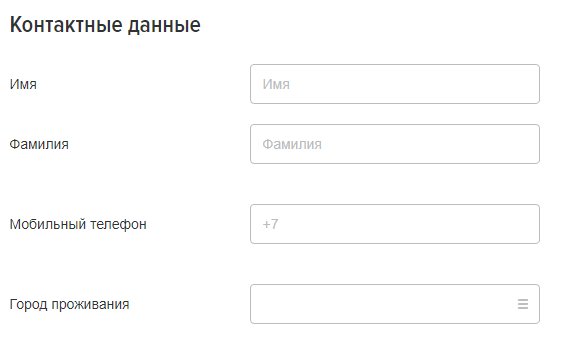
\includegraphics[width=12cm]{images/image14.png}
            \caption{\label{fig:1}%
                Структура пункта контактных данных}
        \end{figure}

    \item Заполнить пункты основной информации. Структура пункта представлена на рисунке~\ref{fig:2}.
        \begin{figure}[!ht]
            \centering
            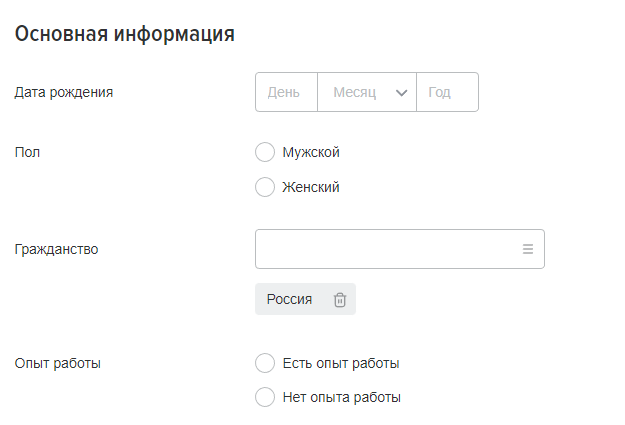
\includegraphics[width=12cm]{images/image12.png}
            \caption{\label{fig:2}%
                Структура пункта основной информации}
        \end{figure}

    \item Указать желаемую специальность и заработную плату. Структура пункта представлена на рисунке~\ref{fig:3}.
        \begin{figure}[!ht]
            \centering
            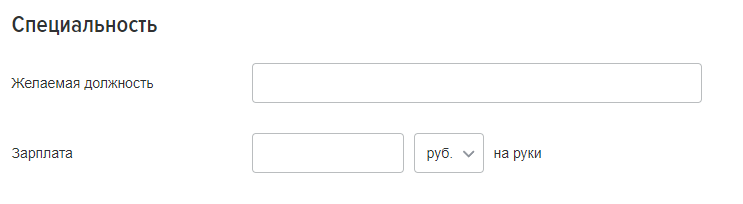
\includegraphics[width=12cm]{images/image3.png}
            \caption{\label{fig:3}%
                Структура пункта специальности}
        \end{figure}

    \item Указать опыт работы (при его наличии), а также навыки, которые предлагаются пользователю в качестве отдельных ключевых слов;
    \item Указать уровень образования, место его получения и года выпуска (либо <<по настоящее время>> для школьников или студентов);
    \item Указать владение языками и его уровень (для иностранных). Структура пункта представлена на рисунке~\ref{fig:4}.
        \begin{figure}[!ht]
            \centering
            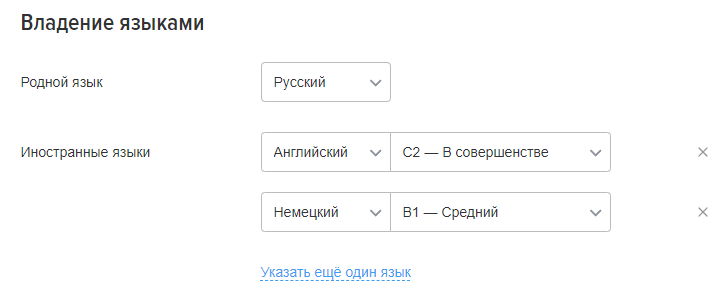
\includegraphics[width=12cm]{images/image1.png}
            \caption{\label{fig:4}%
                Структура пункта владения языками}
        \end{figure}
    \item Пункт <<другой важной информации>> содержит в себе сведения о готовности к переезду, желаемой занятости, графика работы, наличии автомобиля и водительских прав, а также категорий в них. Для иностранных граждан присутствует пункт <<разрешения на работу>>.
\end{enumerate}

После публикации резюме его может быть не видно большинству работодателей, если некоторые из пунктов являются незаполненными. Сам алгоритм составления резюме не является сложным, а возможность откликнуться на вакансию часто подразумевает прикрепление сопроводительного письма помимо самой <<визитки>> соискателя. Дополнительно сервис hh.ru предлагает услуги экспертов для составления грамотного резюме за небольшую плату (от 3 до 8 тысяч рублей в зависимости от разновидности услуги).

\subsection{Сервис для поиска работы в IT-сфере Хабр Карьера}
Являясь одним из популярных в России коллективным IT-блогом, Хабр смог развить не только форум для программистов, но и отдельные сервисы, которые связаны с помощью начинающих и опытных разработчиков, тестировщиков, дизайнеров и прочих информационных вакансий. Одним из подобных сервисов для поддержки начинающих и опытных IT-специалистов является Хабр Карьера\cite{Gridneva_2021}.

В отличие от hh.ru, Хабр Карьера публикует вакансии исключительно связанные с IT сферой. На сервисе предлагаются вакансии как небольших компаний, так и компаний-гигантов (например, Яндекс, Авито, Mail.ru). Для своих коллег и знакомых на Хабр Карьера пользователю предоставляется возможность оставить профессиональную рекомендацию.

Составление резюме на сайте начинает свой путь с процесса авторизации на сервисе. Это можно сделать как при помощи стандартной регистрации с подтверждением почты, так и через сервисы, доступные в России (Вконтакте, Google Account).

Составить своё резюме Хабр Карьера предлагает сразу же после авторизации, причём существует возможность импортировать резюме с сервиса hh.ru. Данное окно представлено на рисунке~\ref{fig:5}.
\begin{figure}[!ht]
    \centering
    
\includegraphics[width=12cm]{images/image9.png}
    \caption{\label{fig:5}%
        Предложение импорта резюме с hh.ru}
\end{figure}


Для ручного ввода или создания первого резюме пользователю потребуется 3 шага:
\begin{enumerate}
    \item На первом указывается фамилия и имя, пол и дата рождения, а также основная цель регистрации на Хабр Карьера. Структура пункта представлена на рисунке~\ref{fig:6}.
    \begin{figure}[!ht]
        \centering
        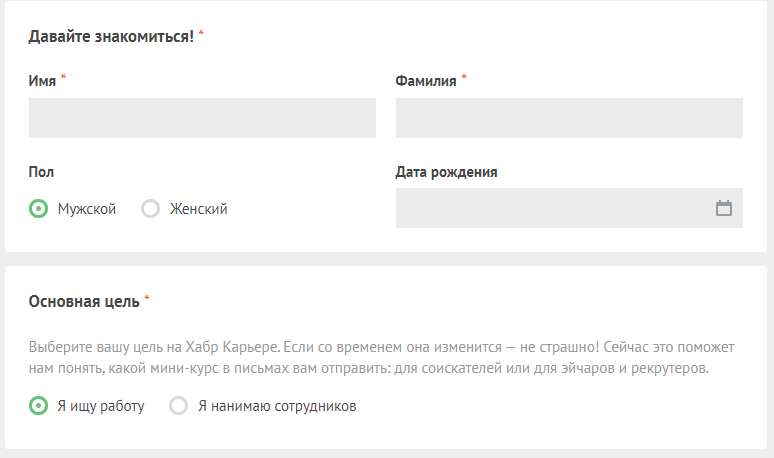
\includegraphics[width=12cm]{images/image15.png}
        \caption{\label{fig:6}%
            Первый шаг регистрации}
    \end{figure}
    В той же вкладке (если выбрана роль соискателя) необходимо выбрать основную специализацию и отдельный профиль, а также квалификация (Intern, Junior, Middle, Senior, Lead). В отличие от hh.ru и в связи с ограниченной сферой деятельности, все специализации представлены наглядно и распределены по категориям для удобства выбора. Дополнительно указываются профессиональные навыки, которым владеет соискатель. Список таких навыков очень обширен и позволяет гибко найти нужные профессиональные <<скиллы>>. Часть из них предлагается уже на старте как <<Самые популярные>>. Структура пункта представлена на рисунке~\ref{fig:7}.
    \begin{figure}[!ht]
        \centering
        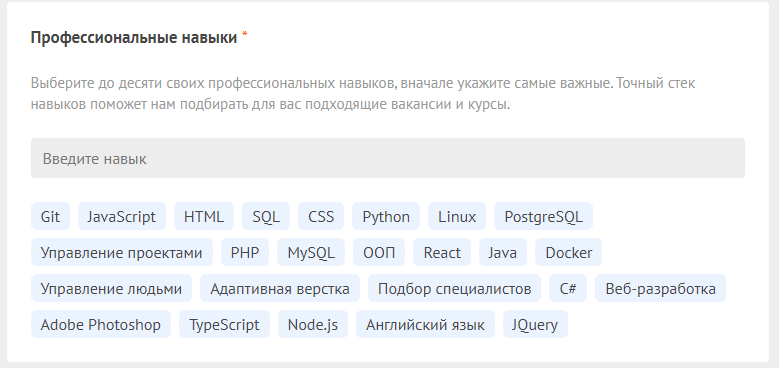
\includegraphics[width=12cm]{images/image19.png}
        \caption{\label{fig:7}%
            Выбор профессиональных навыков}
    \end{figure}

    \item Вторая вкладка будет содержать в себе контактную информацию, что также важно при составлении резюме, ведь одних данных об имени и фамилии будет недостаточно для связи с соискателем. По содержанию оно аналогично сервису hh.ru, например, указать город проживания и пункт о готовности к переезду или удаленной работе. Однако для связи соискатель может оставить не только номер телефона или ссылку-портфолио, но и свой логин в мессенджерах, например, в Telegram. Структура пункта представлена на рисунке~\ref{fig:8}.
    \begin{figure}[!ht]
        \centering
        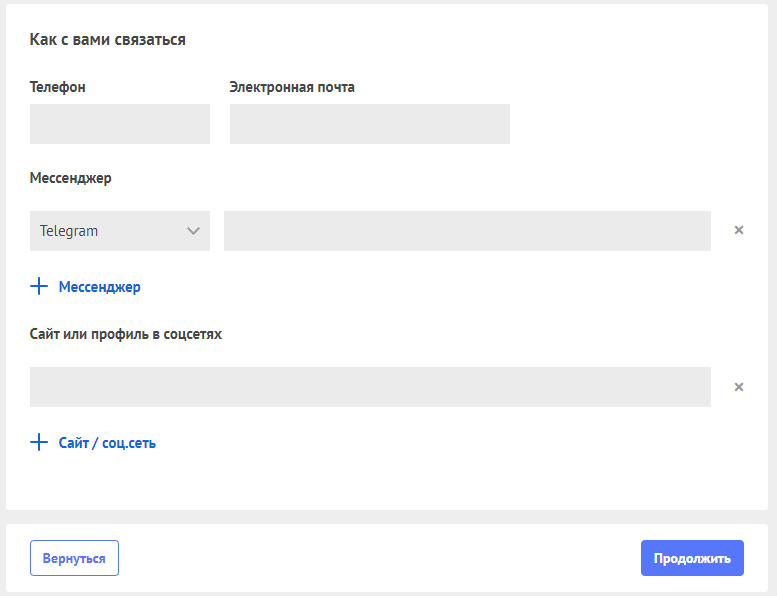
\includegraphics[width=12cm]{images/image2.png}
        \caption{\label{fig:8}%
            Выбор контактных данных}
    \end{figure}

    \item Последняя вкладка содержит в себе пункты, связанные с опытом работы. По статистике, большинство работодателей присматриваются к кандидатам, у которых за спиной есть даже самый незначительный, но указанный в резюме опыт. Однако на Хабр Карьера отсутствует пункт, связанный с <<фрилансом>>, что мешает заполнению опыта работы в данной сфере, но его можно добавить самостоятельно.
\end{enumerate}

\subsection{Международный сервис поиска работы Skipp.dev}
Skipp.dev является международным сервисом как для поиска работы, так и для найма работников со стороны работодателей. Различие между предыдущими сервисами отличается не только в плане дизайна, но и порядка заполнения пунктов. Для того, чтобы начать поиск желаемой вакансии, необходимо также пройти авторизацию, и после этого поочередно заполнить пункты специализации и навыков:
\begin{enumerate}
    \item Необходимо верифицироваться по номеру мобильного телефона. Этот пункт необходим для того, чтобы проверить подлинность аккаунта, а также для дальнейшей авторизации на сервисе при помощи смс-кода.
    \item На первом шаге соискателю предлагается выбрать свои навыки. Структура пункта представлена на рисунке~\ref{fig:9}.
        \begin{figure}[!ht]
            \centering
            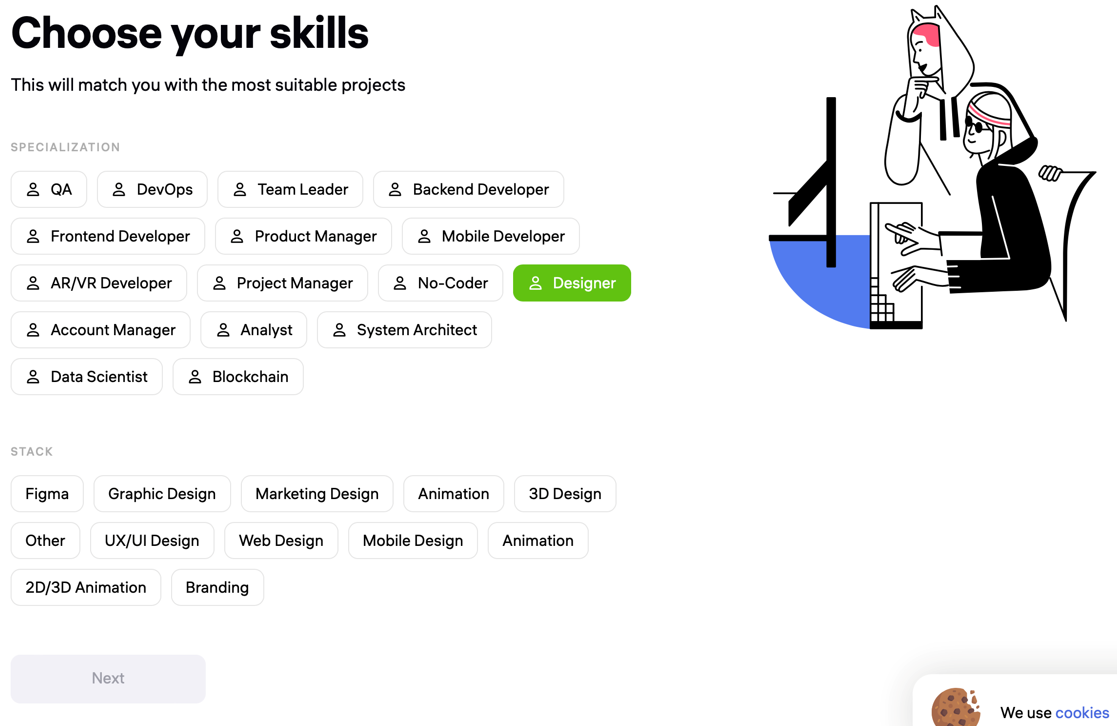
\includegraphics[width=12cm]{images/image10.png}
            \caption{\label{fig:9}%
                Выбор навыков}
        \end{figure}
    \item После выбора навыков необходимо указать уровень навыков, которые были выбраны на предыдущей странице, что является нестандартным для отечественных сервисов. Структура пункта представлена на рисунке~\ref{fig:10}.
    \begin{figure}[!ht]
        \centering
        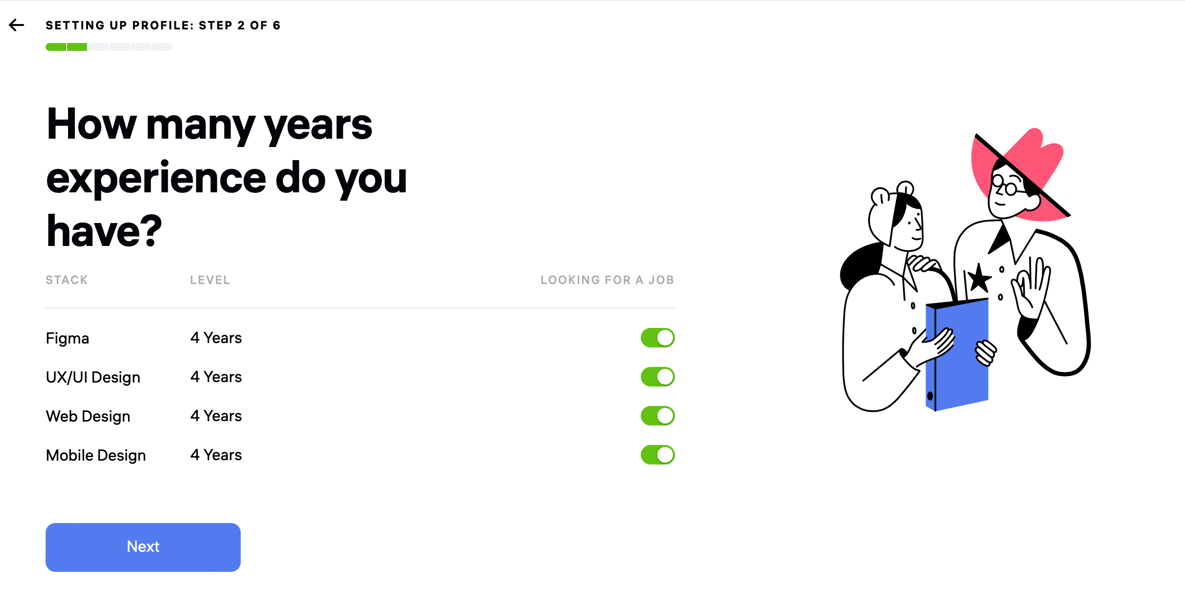
\includegraphics[width=12cm]{images/image11.png}
        \caption{\label{fig:10}%
            Выбор уровня навыков}
    \end{figure}

    \item Заполнение опыта работы не сильно отличается от рассмотренных нами предыдущих платформ, но имеет свои преимущества. Например, для более подробного описания должностных обязанностей на предыдущих местах работы пользователю предлагаются различные виды деятельности, также начиная с самых популярных на сайте. Также к опыту работы есть возможность приложить изображения в качестве портфолио. Структура пункта представлена на рисунке~\ref{fig:11}.
    \begin{figure}[!ht]
        \centering
        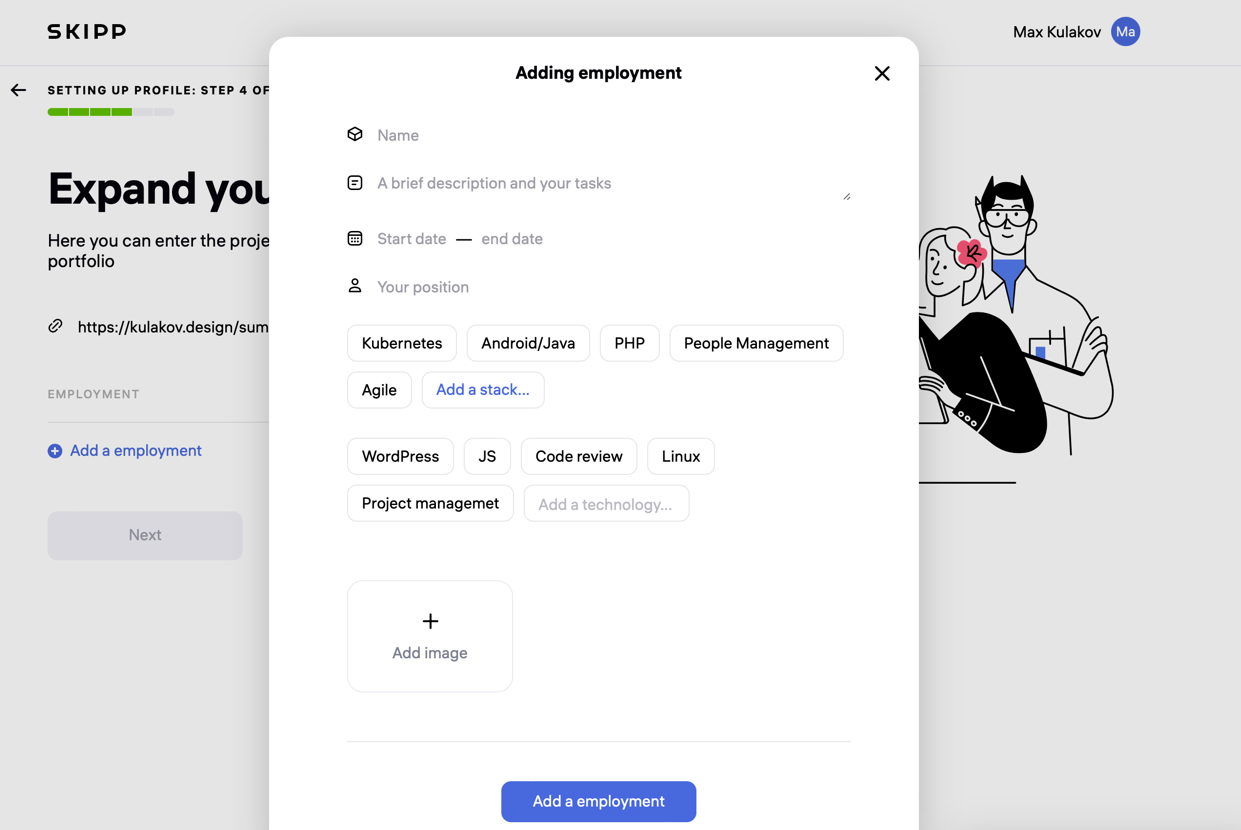
\includegraphics[width=12cm]{images/image17.png}
        \caption{\label{fig:11}%
            Выбор опыта работы}
    \end{figure}

    \item Последний пункт содержит в себе форму заполнения контактной информации, начиная от ФИО до номера телефона и e-mail. 
\end{enumerate}

Из положительных сторон данного сервиса можно выделить приятный внешний вид и неторопливое пошаговое заполнение всех пунктов. Акцент делается на опыте работы, чтобы сконцентрировать внимание пользователя на том, как будет лучше преподнести себя будущим работодателям. Однако сервис не захватывает резюме с других платформ, что делает эту платформу абстрагированной от других себе подобных.

\subsection{Карьерный ресурс Icanchoose}
ICanChoose рекомендует себя в качестве карьерного ресурса нового формата. Из новизны, предполагаемо, сервис предлагает помощь в поиске работы, а также предлагает карьерные советы.

Авторизация на сервисе доступна при помощи ВКонтакте, а так же с email. При создании резюме сразу предлагается импорт из сервиса hh.ru, представленный на рисунке~\ref{fig:12}.
\begin{figure}[!ht]
    \centering
    
\includegraphics[width=12cm]{images/image13.png}
    \caption{\label{fig:12}%
        Возможность импорта резюме}
\end{figure}

Процесс составления резюме происходит так же, как на вышерассмотренных сервисах, но с добавлением пунктов о хобби, достижениях и сопроводительное письмо. Также на сервисе существует возможность предварительного просмотра готового резюме, которое работает только при полном заполнении основной информации.

\subsection{Веб-сервис для хостинга ГитХаб}
ГитХаб зарекомедовал себя крупнейшим сервисом для хостинга с возможностью их совместной разработки, но, благодаря своим инструментам, на платформе возможно создание резюме. На аккаунте начинающего разработчика такое решение будет являться хорошим продолжением стратегии его развития, так как при рассмотрении профиля в качестве портфолио работодателю будут видны все разработанные проекты, на основе чего высока вероятность получить приглашение самому разработчику.

Для начала работы с составлением резюме пользователю необходимо создать новый репозиторий с названием, которое будет повторять <<юзернейм>> на GitHub. Сервис подчеркнёт его в качестве уникального и захватит его нужным образом.

Вся информация по резюме будет находиться в файле README.md. Другими словами, всё написанное и отформатированное будет видно на странице в GitHub и будет служить в дальнейшем красочной визиткой для тех, кто будет просматривать профиль разработчика\cite{gh_cv}.

Удобство написания резюме в GitHub подкрепляется отсутствием шаблона и полной свободой мысли, однако из-за отсутствия точных критериев содержания информации необходимо для себя составлять структуру будущей визитки, чтобы она выглядело не только гармонично, но и понятно.

\subsection{Блочный конструктор веб-сайтов Tilda}
Tilda изначально является конструктором, позволяющиим на внутренних шаблонах создать любой сайт, который удовлетворяет задаче, в том числе резюме. Для последнего на сайте есть готовые шаблоны, которые упрощают работу с сервисом, в частности для начинающих пользователей\cite{tilda_template}. Визуально это представлено на рисунке~\ref{fig:13}.
\begin{figure}[!ht]
    \centering
    
\includegraphics[width=12cm]{images/image7.png}
    \caption{\label{fig:13}%
        Предложение использования шаблона}
\end{figure}

Составленный из блоков шаблон также можно будет использовать в качестве собственного лендинга.

Профиль на Тильде также является портфолио, что позволяет работодателю, желающему создать сайт на данном сервисе, найти необходимого ему разработчика при помощи системы заказов на Tilda Express.

Резюме на Tilda Express представляет из себя небольшую страницу с размещенными на них проектами, разработанными на Tilda, а также окошком с заполнением заявки на обратную связь при наличии желания заказать у данного разработчика собственный сайт. Пример резюме представлен на рисунке~\ref{fig:14}.
\begin{figure}[!ht]
    \centering
    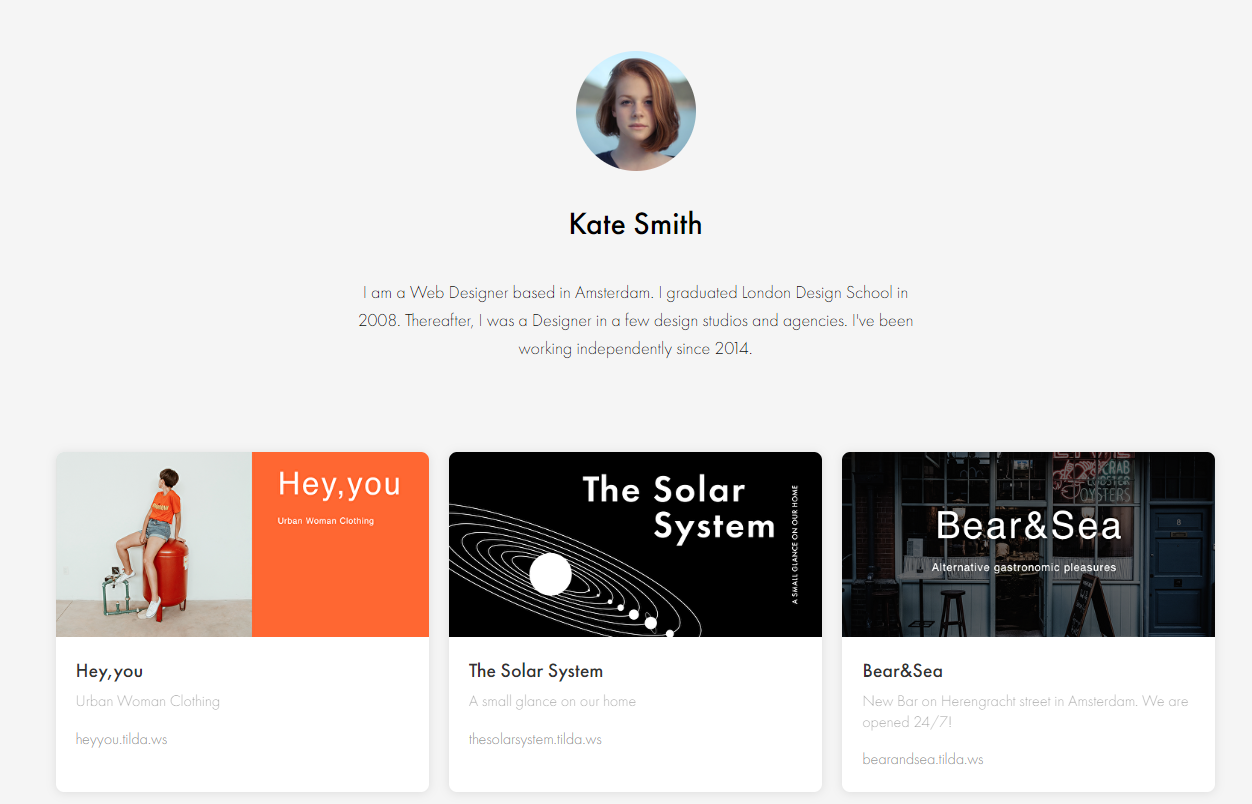
\includegraphics[width=12cm]{images/image8.png}
    \caption{\label{fig:14}%
        Пример резюме на платформе Tilda}
\end{figure}

\subsection{Онлайн-конструктор резюме Simpledoc}
SimpleDoc является сервисом исключительно по составлению резюме. На сайте предлагается составление резюме в трёх основных этапах: заполнение формы, выбор дизайна для резюме и его скачивание или отправка по e-mail, представленных на рисунке~\ref{fig:15}.
\begin{figure}[!ht]
    \centering
    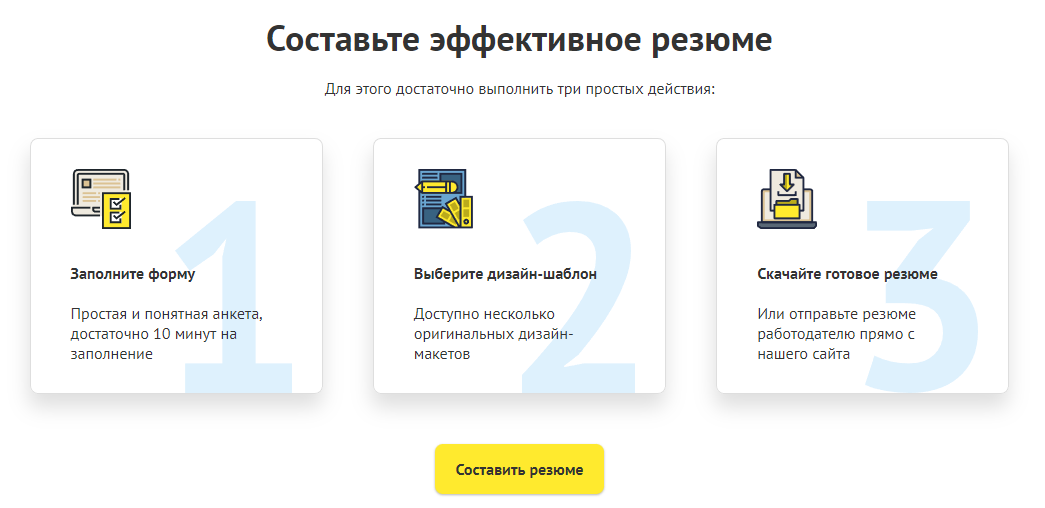
\includegraphics[width=12cm]{images/image5.png}
    \caption{\label{fig:15}%
        Этапы создания резюме}
\end{figure}

Сам процесс заполнения формы занимает около 10ти минут и содержит в себе стандартные для резюме пункты:
\begin{enumerate}
    \item Основная информация;
    \item Личная информация;
    \item Опыт работы;
    \item Образование;
    \item Курсы и тренинги;
    \item Иностранные языки и компьютерные навыки;
    \item Дополнительная информация.
\end{enumerate}

После заполнения пунктов сервис предлагает выбрать один из четырёх шаблонов для дальнейшего скачивания, представленных на рисунке~\ref{fig:16}.
\begin{figure}[!ht]
    \centering
    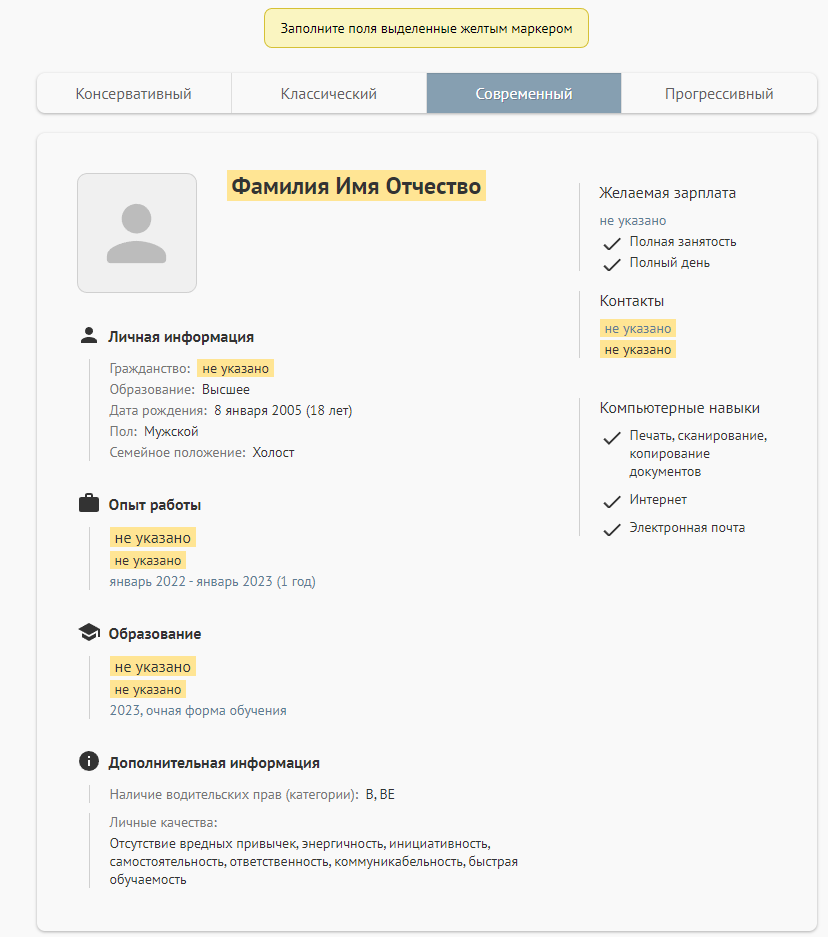
\includegraphics[width=12cm]{images/image4.png}
    \caption{\label{fig:16}%
        Вариант шаблона резюме}
\end{figure}

После составления резюме по шаблону пользователь сможет скачать его и редактировать в течение месяца после разовой оплаты на самом сервисе. Сервис также не позволяет импортировать резюме с других сервисов.

\subsection{Онлайн-конструктор Enhancv}
Enhancv также является сервисов для составления резюме, но в отличие от SimpleDoc имеет приятный дизайн, представленный на рисунке~\ref{fig:17} уже со стартовой страницы:
\begin{figure}[!ht]
    \centering
    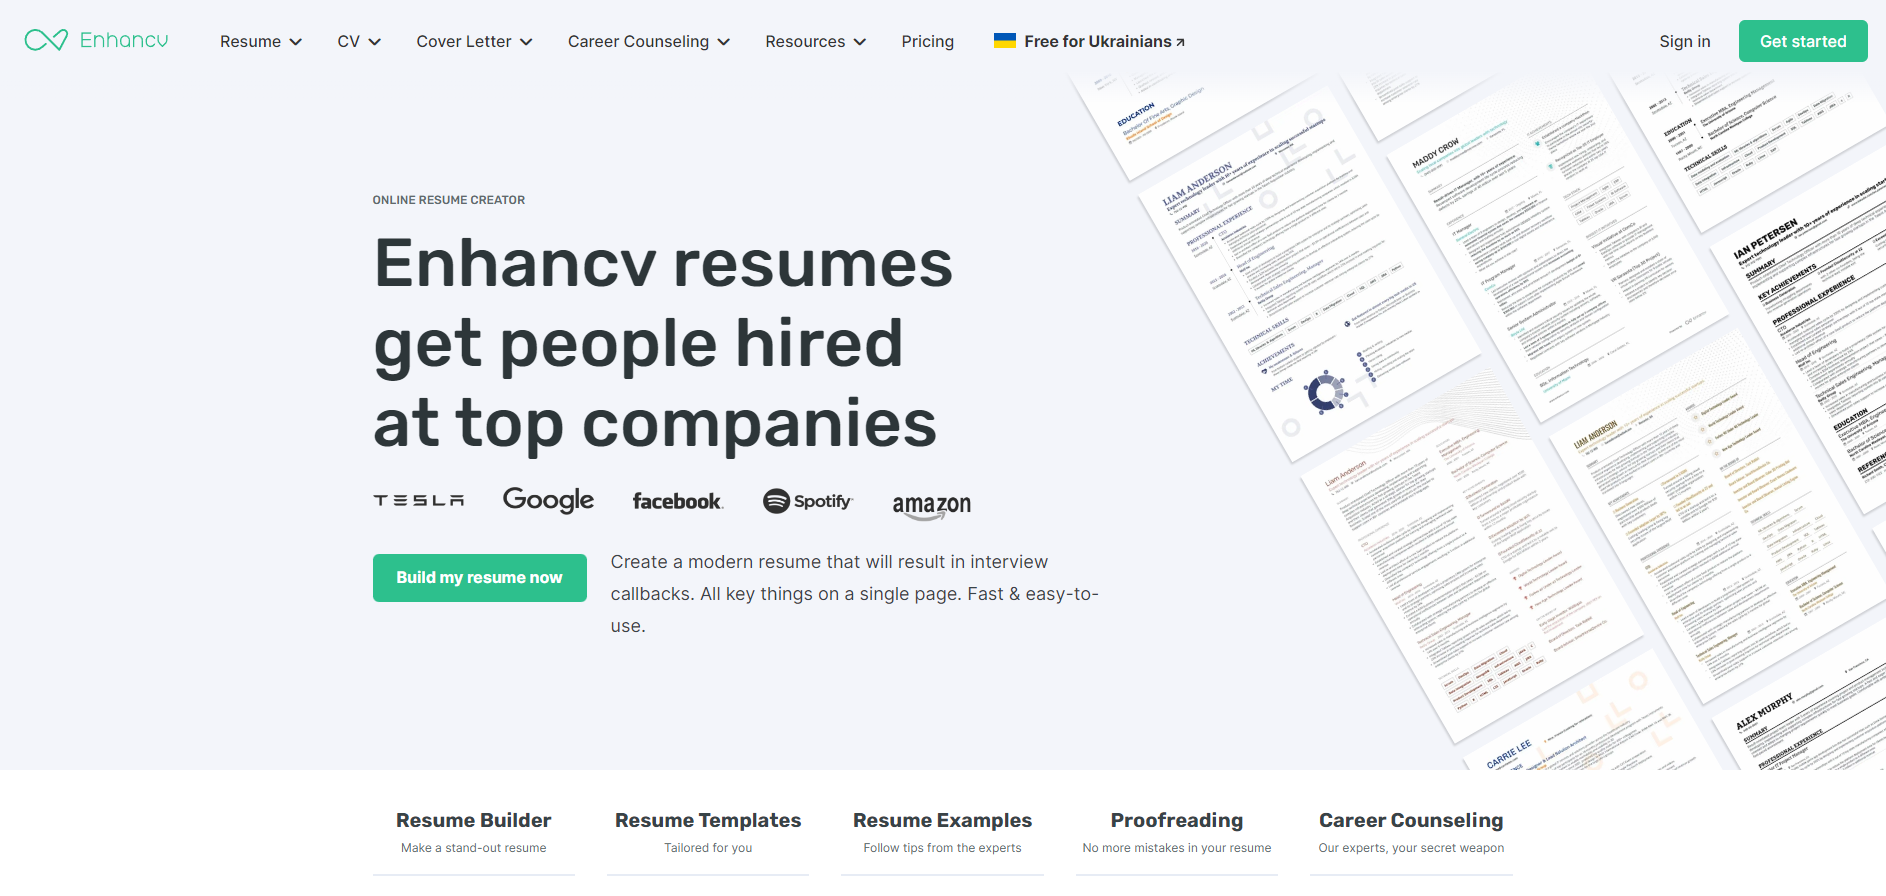
\includegraphics[width=12cm]{images/image18.png}
    \caption{\label{fig:17}%
        Внешний вид сервиса Enhancv}
\end{figure}

При начале работы нам помогает <<виртуальный>> помощник, показанный на рисунке~\ref{fig:18}, с которым мы заполняем пункты по очереди:
\begin{enumerate}
    \item Имя Фамилия
    \item Наличие опыта в создании резюме (для возможности его импортировать)
    \item Готовые шаблоны для будущего резюме.
\end{enumerate}

\begin{figure}[!ht]
    \centering
    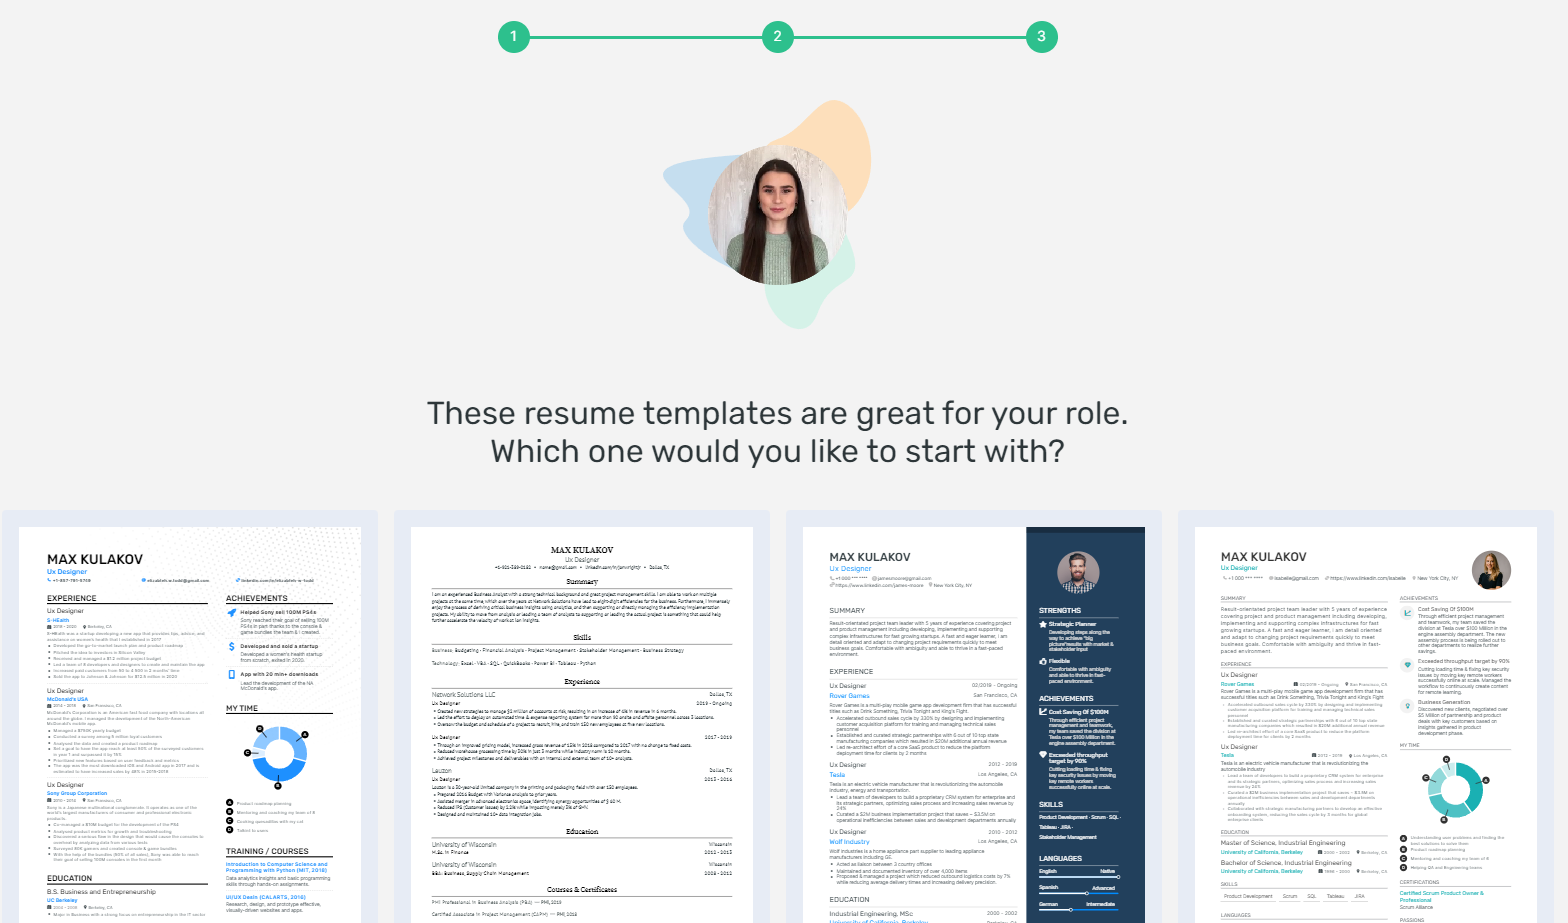
\includegraphics[width=12cm]{images/image16.png}
    \caption{\label{fig:18}%
        Помощник в составлении резюме}
\end{figure}

После чего предлагается отредактировать информацию в резюме напрямую в одном из шаблонов, показанном на рисунке~\ref{fig:19}:
\begin{figure}[!ht]
    \centering
    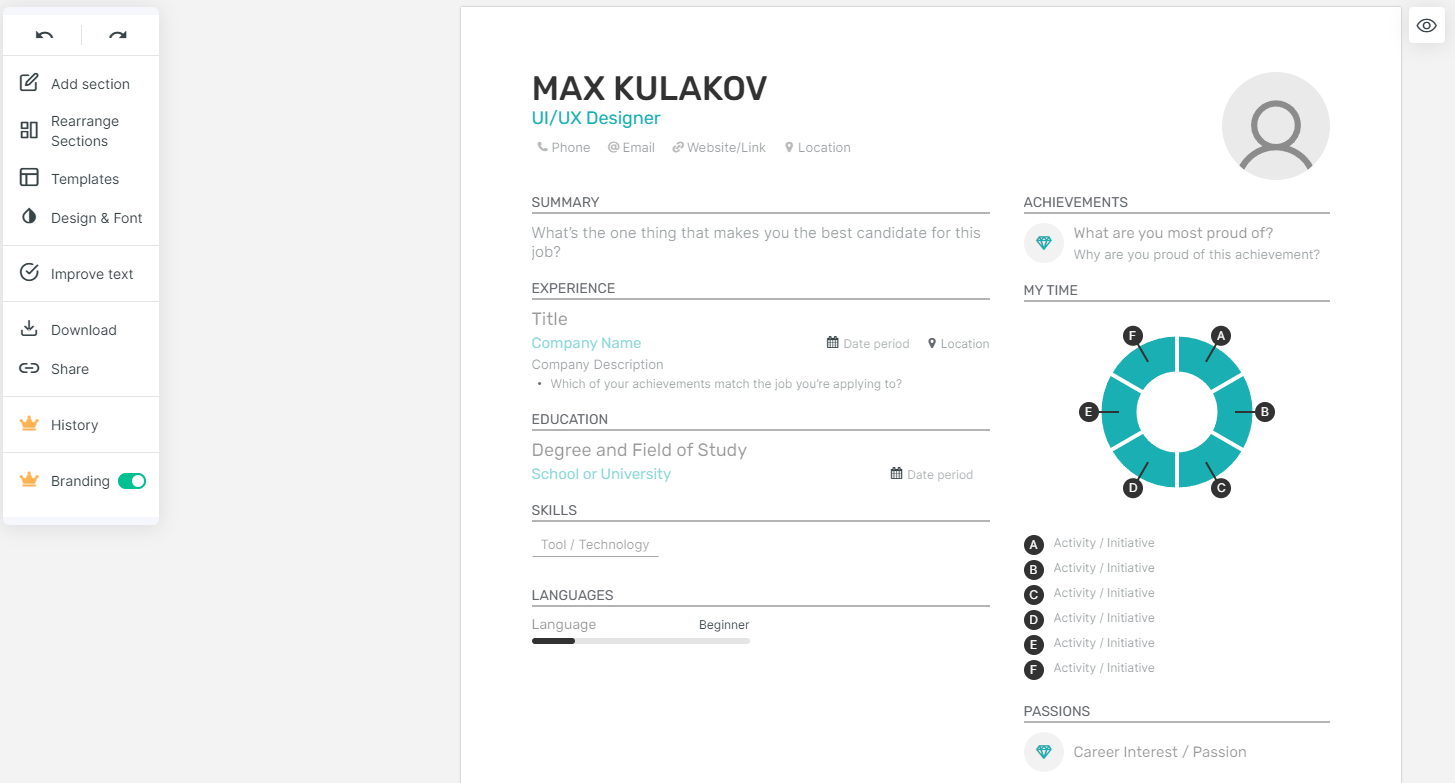
\includegraphics[width=12cm]{images/image20.png}
    \caption{\label{fig:19}%
        Внешний вид шаблона резюме}
\end{figure}

На выбор предлагается множество инструментов для комфортной работы с шаблоном: от возможности редактирования шрифта до редактируемой инфографики. Также является платным сервисом.

На основе просмотренных конкурентных платформ можно вынести их основные недостатки:
\begin{enumerate}
    \item Не все сервисы предлагают импорт резюме из других платформ;
    \item Сервисы, работающие исключительно на составление резюме, берут деньги за свои услуги;
    \item Некоторые сервисы при указании опыта работы требуют официальное название компании или должности, даже если они не зарегистрированы, и не всегда удается указать нужное название;
    \item В дополнение к пункту 3, не везде возможно указание опыта <<свободных заказов>> вне сервисов по типу <<Фриланс.ру>>
    \item Для русскоязычного сегмента сервисов поиска работы основным является именно HeadHunter, импорт резюме с которого предлагается лишь в части платформ.
\end{enumerate}






\newpage
\section{Теоретические аспекты разработки}
\subsection{Интерфейсная библиотека React JS}
React JS - это библиотека JavaScript с открытым исходным кодом, которая предназначена для разработки пользовательских интерфейсов веб-приложений, особенно для интерактивных веб-страниц. Она позволяет использовать "компоненты", которые являются маленькими блоками кода, для создания сложных пользовательских интерфейсов.

React JS прост и удобен в эксплуатации. Понимание основных требований практически не требует времени и может быть выполнено в течение нескольких часов. Разработчики предпочитают использовать React JS по следующим причинам:
\begin{enumerate}
    \item Динамические приложения требуют более сложного кодирования, и использование React JS упрощает данную задачу;
    \item Возможность повторного использования компонентов. В React очень тесно связаны разметка и логика, благодаря чему появляется возможность хранить все данные о внешнем виде компонента и его изменения в процессе работы в одном файле;
    \item Использование виртуального дерева вместо физического для повышения производительности будущего приложения. Для JavaScript структура dom-дерева является интерфейсом, через который скрипты приводят в движение html и css-объекты, поэтому производительность в данном случае играет очень значимую роль;
    \item Снижается нагрузка на сервер и время разработки. Повышается производительность сайта: быстрее открываются страницы и отзывается на действия пользователей интерфейс;
    \item По сравнению с обычными сайтами у сайтов на React более чистая архитектура, в которой проще обнаруживать и исправлять баги и которую проще поддерживать. \cite{rjs_vs_rn}\cite{rjs}
\end{enumerate}

Фреймворк React использует JSX, расширение для языка JavaScript, представляя все HTML-элементы интерфейса в роли компонентов, используя подход «разделяй и властвуй», упрощая разработку проекта, особенно удобно для командной разработки. Подобный подход используется во всех современных фреймворках для разработки динамического web-интерфейса\cite{Ershov_web}.

React очень удобно рассматривать для разработки одностраничных приложений. Несмотря на то, что при снятии нагрузки с сервера нагружается его клиентская часть, современные браузеры способны справиться с отрисовкой страниц благодаря достаточному запасу памяти и подхода SPA. Его суть в том, что весь сайт — это одна страница, которую React постоянно перерисовывает – но не целиком. Если в одностраничных страницах есть возможность оптимизации ресурсов, то и в многостраничных решениях оно будет присутствовать вдоволь.

В простом приложении для перехода со страницы на страницу пользователь делает к ней запрос на сервер, и сервер возвращает разметку, стили и файлы скриптов. В случае одностраничных приложений пользователь, переходя между разделами сайта, формально находится на одной и той же странице, но файлы скриптов и стили у него уже есть — остается догрузить то, чего не хватает. 

По состоянию на конец 2023 года React находится в лидирующих позициях среди JavaScript-технологий для разработки фронтенда\cite{rjs}.



\subsection{Серверная библиотека NextJS}
Переходя к основоположникам применения серверных компонентов можно отнести создателей средства Next.js, развивающих упомянутую концепцию. Next.js – это фреймворк, основанный на React, который позволяет создавать веб-приложения с улучшенной производительностью, используя рендеринг на серверной стороне\cite{Cheprasov2023}.

Дополнительный функционал NextJS обеспечивает реализацию оптимизированных и полезных возможностей, таких как:
\begin{enumerate}
    \item Server Side Rendering – позволяет рендерить полноценную страницу на сервере, после чего она полностью отправляется на клиентскую часть и сразу же отображается, что повышает производительность веб-страниц;
    \item Search Engine Optimization – помогает веб-приложению занимать более высокие места в поисковых системах. SEO работает в тандеме с SSR и позволяет трекерам сканировать больше контента;
    \item Упрощенный процесс разворачивания приложения\cite{Nikitin_nextjs}.
\end{enumerate}

Next.js может быть использован для разработки клиент-серверных приложений с улучшенной производительностью и возможностью использования серверного рендеринга. В качестве фреймворка, основанного на React, Next.js предоставляет средства для создания веб-приложений, которые взаимодействуют с сервером. Он обеспечивает серверный рендеринг, что означает, что приложение может получить полноценную HTML-страницу на сервере и отправить ее на клиентскую сторону для отображения. Это позволяет повысить производительность сайта и улучшить SEO-оптимизацию.

Следовательно, основные подходы к использованию Next.js для разработки клиент-серверных приложений включают в себя применение серверного рендеринга для оптимизации производительности, управление маршрутизацией, обработку данных на стороне сервера, а также управление локальным состоянием приложения.



\subsection{Интерфейсная библиотека TailWind}
Tailwind CSS является набирающим популярность CSS-фреймворком, который дает возможность вносить изменения в оформление сайтов и приложений, не покидая HTML-разметку, в том числе и в компонентах React, не используя тег style. Эти служебные классы позволяют инкапсулировать общие шаблоны стилей, такие как поля, отступы, цвета и макеты флексбоксов, что позволяет быстро создавать и настраивать пользовательский интерфейс\cite{Tailwind}.

Одним из ключевых преимуществ является гибкость и расширяемость. Фреймворк предоставляет широкие возможности настройки, позволяющие разработчикам настраивать структуру в соответствии с конкретными требованиями проекта. Эта гибкость делает его подходящим для широкого спектра проектов: от небольших личных веб-сайтов до крупномасштабных корпоративных приложений.

Tailwind CSS является его ориентация на производительность и оптимизацию. Используя служебные классы, разработчики могут избежать раздувания, которое часто возникает при использовании традиционных платформ CSS, что приводит к меньшим размерам файлов CSS и более быстрому времени загрузки. Более того, поощряет модульный подход к стилизации, который может привести к созданию более удобных в обслуживании и масштабируемых баз кода.

Несмотря на свой подход, ориентированный на полезность, Tailwind CSS не жертвует гибкостью дизайна. Платформа предоставляет полный набор служебных классов, которые охватывают широкий спектр вариантов стилей, что позволяет разработчикам с легкостью создавать визуально привлекательные и адаптивные проекты. Кроме того, Tailwind CSS легко интегрируется с популярными интерфейсными платформами, такими как React, Vue.js и Angular, что упрощает его включение в существующие проекты\cite{Fain_2022}.

Основными преимуществами TailWind CSS являются следующие возможности:
\begin{enumerate}
    \item Наличие базовых классов для оформления страниц. В библиотеке есть базовый конфигурационный файл, и в него по умолчанию включена большая коллекция классов, необходимых для стилизации приложения, таких как flex, grid, block для display, m-10 вместо margin и подобных;
    \item Наличие расширенной цветовой палитры. Цвета здесь имеют привычные названия и постфикс с насыщенностью в цифровом обозначении, например, red-50 будет являться бледно-розовым цветом, когда red-900 уже приобретет более бордовый оттенок;
    \item Продвинутые CSS-свойства. Различные анимации, радиусы закругления рамок, повороты, отступы;
    \item Переменные. Помимо классов, в Tailwind CSS есть и переменные в стиле тех, что используется в CSS-препроцессорах. С помощью них можно уложить несколько классов в один и использовать его как классический семантический селектор. Делается это с помощью директивы @apply;
    \item Добавление собственных классов. В этом плане Tailwind можно настроить под индивидуальные требования и предпочтения. Для этого требуется прописать новые свойства в конфигурационный файл фреймворка\cite{Tailwind}.
\end{enumerate}

Подводя итог, Tailwind CSS предлагает современный и эффективный подход к стилизации веб-приложений. Благодаря своей философии приоритета полезности, широким возможностям настройки и ориентации на производительность дает разработчикам возможность создавать красивые и отзывчивые пользовательские интерфейсы с меньшими усилиями и большей гибкостью\cite{Rifandi_2022}. 



\subsection{Архитектурный стиль Rest API}
Rest API - это интерфейс программирования приложений, основанный на принципах REST. Web API или Web Service API –это интерфейс обработки приложений между веб-сервером и веб-браузером. Все веб-сервисы являются api, но не все api являются веб-сервисами. Rest API – это особый тип Web API, в котором используется стандартный архитектурный стиль, описанный выше\cite{Kalinin_mic}.

Различные термины, которые относятся к API, например, Java API или сервисные API, существуют в связи с исторически ранним происхождением, тк API-архитектуры начали появляться до запуска Всемирной паутины. Современные web API – это REST API, и эти термины могут использоваться взаимозаменяемо.

Данный архитектурный стиль стал популярным из-за своей простоты, гибкости и масштабируемости. Он использует стандартные HTTP-методы, такие как GET, POST, PUT и DELETE, для работы с ресурсами на сервере. Каждый ресурс имеет уникальный идентификатор, с которым клиенты могут взаимодействовать.

В качестве основных преимуществ архитектурного стиля Rest API можно выделить следующие ключевые моменты:
\begin{enumerate}
    \item Гибкость – позволяет разработчикам использовать различные форматы данных, такие как json или html. Это позволяет клиентам и серверам обмениваться данными в удобном для них формате;
    \item Простота – использует стандартные HTTP-методы, что делает его простым в использовании и понимании. Разработчики могут легко создавать, изменять и расширять api без необходимости в специальных инструментах или библиотеках;
    \item Масштабируемость – позволяет разрабатывать распределенные системы, где клиенты и серверы могут находиться на разных компьютерах или даже в разных частях мира. Это делает его идеальным для создания клиент-серверных приложений;
    \item Кэширование – поддерживает кэширование данных на клиентской стороне, что позволяет улучшить производительность и снизить нагрузку на сервер;
    \item Независимость от платформы – не привязан к определенной платформе или языку программирования. Это означает, что клиенты и серверы могут быть реализованы на различных технологиях, а это уже обеспечивает большую гибкость и возможность использования уже существующих разработанных систем.\cite{Masse_rest}
\end{enumerate}

В настоящее время Rest API является широко используемым и популярным подходом для разработки клиент-серверных приложений, благодаря своей простоте, гибкости, масштабируемости и прочим незаменимым, полезным возможностям.



\subsection{Сервис тестирования API Postman}
Postman — это инструмент, используемый разработчиками для создания, тестирования и документирования API. Его основная особенность заключается в том, что он упрощает каждый этап жизненного цикла API и оптимизирует совместную работу для более качественной API-разработки\cite{postman_what}. Postman позволяет выполнять различные типы HTTP-запросов (GET, POST, PUT, PATCH), сохранять среды для последующего использования, преобразовывать API в код для использования в различных языках (например, JavaScript и Python).

Postman обладает широким спектром инструментов, предназначенных для проведения качественного тестирования различных программных приложений и веб-сервисов. Включая коллекции запросов и удобный механизм ввода параметров, этот функционал существенно облегчает работу тестировщика, позволяя эффективно автоматизировать рутинные задачи и выявлять потенциальные ошибки при взаимодействии с API\cite{Marinchuk_2020}.

Postman предлагает ряд функций, которые упрощают процесс разработки:
\begin{enumerate}
    \item Универсальные методы запросов: Postman поддерживает множество методов HTTP-запросов, включая GET, POST, PUT, DELETE и PATCH. Эта универсальность позволяет разработчикам всесторонне взаимодействовать с API;
    \item Управление окружениями: Postman позволяет создавать разные "окружения" для тестирования API. Так, можно иметь отдельное окружение для разработки, тестирования и продакшна, каждое из которых может использовать разные базы данных или внешние сервисы;
    \item Упрощенная аутентификация: Postman упрощает тонкости аутентификации, обеспечивая поддержку различных методов, таких как ключи API, OAuth и базовая аутентификация. Это упрощает процесс обеспечения взаимодействия API, обеспечивая надежную и безопасную среду разработки;
    \item Автоматизация тестов: Postman предоставляет возможности для написания тестов, которые могут автоматически проверять ответы API на соответствие ожидаемым результатам. Это включает в себя проверку статус-кодов ответов, структуры данных и других ключевых аспектов ответа;
    \item Эффективная документация: Postman хорошо генерирует документацию по API непосредственно из запросов. Эта функция обеспечивает оптимизированный и централизованный подход к документированию API, полезный как для внутренних команд разработчиков, так и для внешних заинтересованных сторон. Процесс документирования является эффективным, обеспечивая ясность и доступность\cite{postman_introduction}.
\end{enumerate}

В качестве основных задач и этапов разработки Postman находит свое применение в веб-приложении, которое используются для проверки и тестировании API. Это веб-приложение ускоряет процесс разработки, так как разработчики могут сразу проверить корректность реализации API. Если при разработке возникают ошибки, Postman позволяет быстро тестировать изменения в API и анализировать ответы, что  помогает находить и устранять проблемы. Postman также поддерживает совместные проекты, позволяя командам разработчиков делиться коллекциями запросов и окружениями, что упрощает совместную работу над API. Для новых сотрудников и сторонних разработчиков наличие хорошо документированных и легко доступных API через  Postman упрощает их понимание и взаимодействие с веб- приложением.Будучи комплексным и удобным для пользователя инструментом, Postman дает разработчикам возможность точно ориентироваться в тонкостях взаимодействия API, способствуя оптимизации рабочего процесса\cite{postman_introduction}.



\subsection{Система управления базами данных MongoDB}
MongoDB представляет из себя документо-ориентированную СУБД, которая долгое время играет значительную роль в разработке веб-приложений. Свою популярность MongoDB получила за счёт высокой производительности, гибкости структур данных, масштабируемости и легкости интеграции с различными платформами и языками программирования.

Модель документа MongoDB проста для изучения и использования разработчиками, но при этом предоставляет все возможности, необходимые для удовлетворения самых сложных требований в любом масштабе:
\begin{enumerate}
    \item Документо-ориентированность: В MongoDB информация хранится в виде документов JSON (BSON - Binary JSON), что делает СУБД гибкой в отношении схем данных. Это позволяет разработчикам легко и быстро модифицировать схему базы данных без необходимости остановки базы данных или затраты больших усилий на миграции данных;
    \item Масштабируемость: MongoDB поддерживает горизонтальное масштабирование через механизм шардирования, позволяющий распределить данные по нескольким серверам. Это может существенно повысить производительность и объём хранилища;
    \item Высокая доступность: СУБД использует модель репликации, обеспечивая автоматическое создание копий данных на различных серверах. Это не только повышает устойчивость и доступность приложения в случае сбоев, но и улучшает время ответа на запросы за счет распределенной обработки\cite{mongodb_what}\cite{data_introduction}.
\end{enumerate}

Что касается разработки веб-приложений, MongoDB активно используется в данном направлении благодаря своей способности быстро обрабатывать большие объемы структурированных и неструктурированных данных. Её документо-ориентированный подход своевременно удовлетворяет требования современных веб-приложений, где может потребоваться изменение структуры данных в силу изменения бизнес-требований или пользовательских предпочтений. Например, это может быть разработка социальных сетей, где требуется хранение большого количества медиафайлов, интернет-магазинов, с применением гибкости схемы СУБД для каталогов с различными атрибутами товаров, и сфера аналитики и Big Data, в которой необходимо поддерживать хранение и быструю обработку информации, в частности для систем с аналитическими запросами в реальном времени. Также MongoDB легко интегрируется с большинством современных технологических стеков и языков программирования, таких как JavaScript (Node.js), Python, Java, PHP, Ruby и других\cite{mongodb_what}\cite{Cockoulin_2022}.

Применение MongoDB в разработке веб-приложений демонстрирует значительные преимущества в управлении гибкостью, масштабируемостью и производительностью. Она подходит для различных типов приложений, от простых веб-сайтов до сложных корпоративных решений. Успешно зарекомендовав себя в мире высоконагруженных интернет-приложений и сервисов, MongoDB остается одним из лидеров среди NoSQL систем управления базами данных.



\subsection{Платформа сборки и управления Docker}
Docker представляет собой инновационную платформу, целью которой является обеспечение эффективной разработки, развертывания и запуска приложений в изолированных контейнерах. Термин "Docker" стал ассоциироваться с концепцией контейнеризации в современной технологической среде. Применение Docker и контейнеризация в целом приобрели ключевое значение в сфере веб-разработки, обеспечивая упаковку и изоляцию приложений с целью оптимизации процессов их развертывания и управления\cite{Beloded_2023}.

Как и стандартный многоразовый пластиковый контейнер, Docker обладает рядом ключевых атрибутов. Внутри контейнера можно хранить различные артефакты, которые могут находиться как в пределах контейнера, так и за его границами. Контейнер Docker мобилен и может быть использован на локальном компьютере или на сервере облачного провайдера, такого как AWS.

Особенности контейнеров Docker включают возможность удобного добавления и извлечения содержимого, а также взаимодействия с внешними средствами. Например, контейнеры обладают портами, которые могут быть открыты для доступа к приложениям через браузер. Работа с контейнерами также возможна с помощью командной строки.

Образы Docker-контейнера сохраняются в специальных репозиториях и могут быть загружены и использованы для создания контейнера по запросу. Используя Docker, можно одновременно запускать несколько контейнеров на одном компьютере, управлять их жизненным циклом, исследовать содержимое и создавать новые контейнеры.

Dockerfile представляет собой файл, содержащий инструкции для сборки образа контейнера. В нем описывается базовый образ, который представляет начальный слой контейнера. Популярные базовые образы включают в себя python, ubuntu, alpine. Помимо базового образа, в образ контейнера можно добавлять дополнительные слои с помощью инструкций из Dockerfile. Например, в случае описания образа для машинного обучения, можно указать инструкции для добавления библиотек NumPy, Pandas и Scikit-learn.

Для запуска контейнера необходим образ контейнера и наличие среды, поддерживающей выполнение команд, создающих контейнер с указанным образом и запускающих его в среде, поддерживающей Docker\cite{docker_documentation}\cite{docker_introduction}.



\subsection{Облачная платформа Vercel}
Облачная платформа Vercel является инновационным инструментом для разработки и развертывания веб-приложений, обладающим рядом преимуществ и возможностей. Она предоставляет разработчикам удобное и эффективное окружение для создания современных веб-приложений, применяя современные технологии и подходы. Главными его преимуществами являются высокая скорость развертывания, автоматическое масштабирование, простота использования и интеграции с различными фреймворками, такими как Next.js и другими. Vercel также обладает встроенной поддержкой CI/CD (непрерывной интеграции и непрерывной доставки), что способствует автоматизации процессов разработки и деплоя приложений\cite{vercel_official}.

Использование платформы Vercel позволяет разработчикам сосредоточиться на создании функциональности приложения, минуя сложности настройки инфраструктуры и управления серверами. Vercel поддерживает различные языки программирования, фреймворки и инструменты, что делает ее универсальным и гибким решением для разработчиков. Платформа обеспечивает автоматическое масштабирование приложения в зависимости от нагрузки, что позволяет эффективно управлять ресурсами и обеспечивать отзывчивость сервиса для пользователей\cite{vercel_official}\cite{Litvincev_2023}.

Разработка веб-приложения на React с использованием Vercel начинается с создания репозитория на GitHub, GitLab или Bitbucket. После подключения репозитория, каждый push кода активирует процесс автоматического развертывания. Если проект использует Next.js, Vercel автоматически определит этот фреймворк и применит оптимизации, специфичные для серверного рендеринга (SSR) или статической генерации (SSG). 

Рассматривая практическое применение Vercel в веб-разработке, чаще всего данный инструментарий используется для реализации следующих категорий проектов:
\begin{enumerate}
    \item Развитие стартапа: Компания-стартап, желающая быстро развернуть и оптимально масштабировать свой веб-проект, может воспользоваться Vercel для размещения MVP (минимально жизнеспособного продукта) и последующего продолжения разработки, периодически внося изменения и обновления через CI/CD. Такие успешные примеры разработки можно увидеть непосредственно на сайте разработчиков Vercel\cite{vercel_mural};
    \item Разработка личного портфолио: Веб-разработчик, стремящийся продемонстрировать свои работы и навыки, может использовать Vercel для хостинга своего личного портфолио. Таким образом, развертывание и поддержка сайта будут минимальными, а работа будет доступна широкой аудитории;
    \item Онлайн-магазин: Для запуска онлайн-магазина, где требуется быстрая загрузка страниц и высокая доступность, команда разработчиков может воспользоваться Vercel, чтобы обеспечить стабильную работу приложения и удобное управление контентом.
\end{enumerate}

Благодаря своим преимуществам, Vercel остается незаменимым инструментом для веб-разработки за последнее время.






% Практическая часть
\section{Основные аспекты разработки платформы единого резюме}
С учётом собранных данных при анализе научной литературы и конкурентных сервисов для разработки собственной платформы единого резюме необходимо придерживаться следующим пунктам:
\begin{enumerate}
    \item Реализовать сбор информации о текущих резюме с уже существующих сервисов;
    \item Предоставить возможность объединения, замены, дополнения или удаления 
    смежных или отсутствующих пунктов данных;
    \item Создание единого бланка с отредактированными или созданными полями, 
    с возможностью хранения их на личном пространстве;
    \item Обновление резюме на сторонних площадках новыми пунктами информации.
\end{enumerate}

Для составления необходимого функционала платформы единого резюме, следует реализовать следующее:
\begin{enumerate}
    \item Удобный пользовательский интерфейс, соответствующий современным web-стандартам 
    и позволяющий пользоваться функционалом сервиса на любом устройстве, поддерживающим 
    работу с браузерами;
    \item Авторизацию пользователей и агрегацию данных на сервере проекта;
    \item Возможность создания пользователем персональной страницы на основе шаблонов, 
    для возможности доступа к актуальному резюме при переходе по ссылке сервиса;
    \item Возможность переноса резюме из стороннего ресурса в шаблон платформы;
    \item Публичное пространство, которое может быть использовано как место просмотра 
    резюме работодателями для предложений о сотрудничестве;
    \item Публикацию серверного проекта на хостинг, поддерживающий динамическое 
    создание и обновление страниц согласно подготовленным данным.
\end{enumerate}



\subsection{Создание прототипа платформы резюме}
Прототипирование – разработка интерактивной модели приложения, симулирующее коммуникацию пользователя с интерфейсом и созданное для тестирования базового функционала. Данный этап необходим чтобы удобно и корректно выстроить логику взаимодействия с продуктом и достижения поставленной задачи.

Для создания прототипа использовано приложение Figma, так как оно является бесплатным (платная версия отличается от бесплатной количеством единовременных редакторов проекта и невозможностью организовать команду) и полностью подходит для реализации данного этапа разработки. Были изображены экраны бланка, страницы ввода и свободногоредактора контента, показанные на рисунке~\ref{fig:20}.

\begin{figure}[!ht]
    \centering
    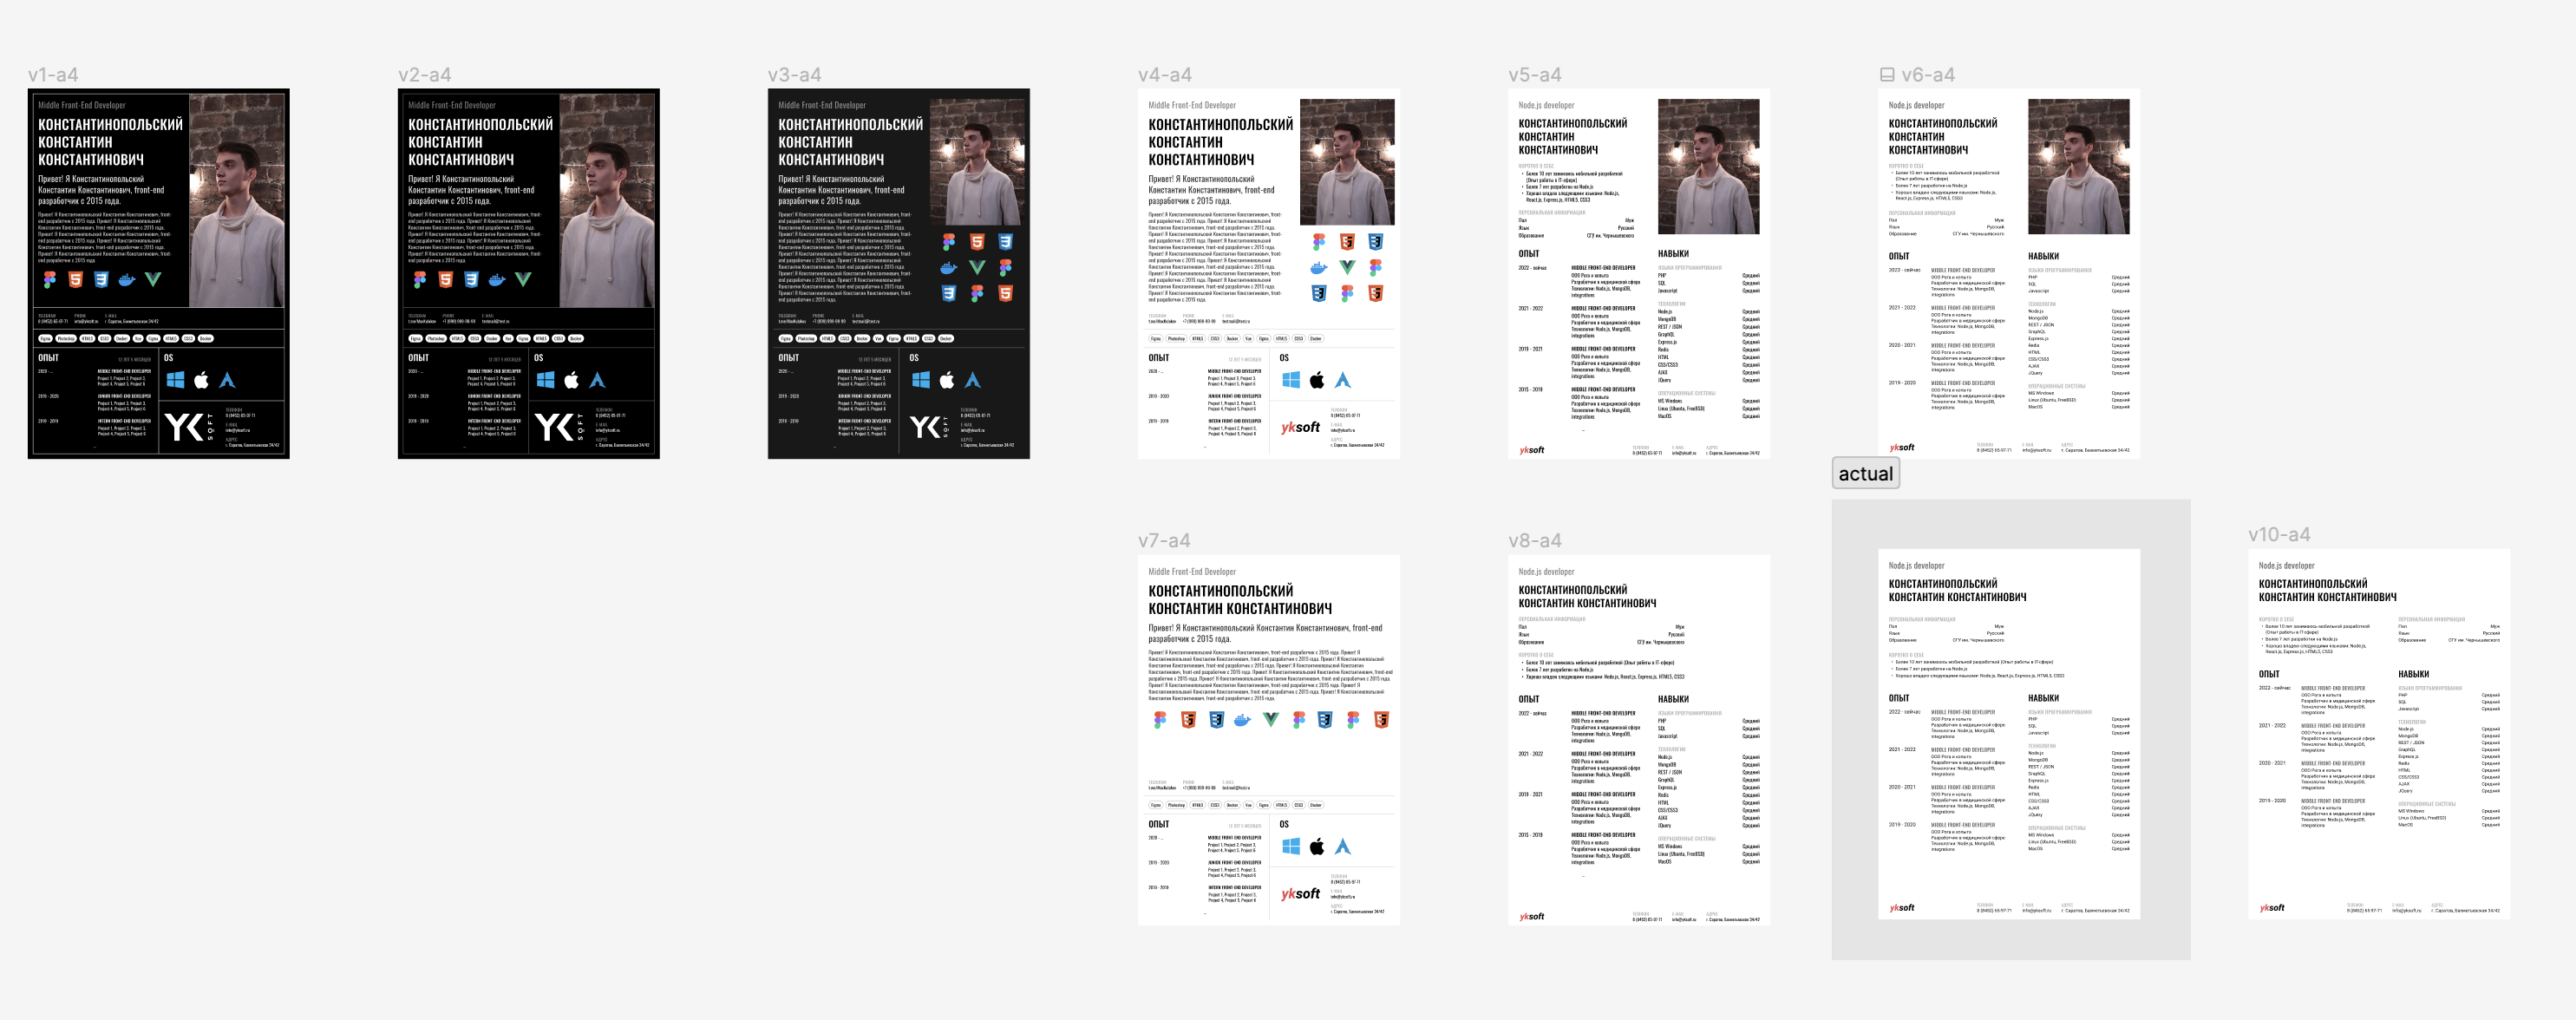
\includegraphics[width=12cm]{images/image21.png}
    \caption{\label{fig:20}%
        Внешний вид прототипов платформы}
\end{figure}

Далее идёт проверка прототипа на реальных людях, проведённая коридорным тестированием – перед случайными людьми ставится задача взаимодействовать с интерфейсом приложения, тогда как разработчик убеждается в корректности задуманного поведения и находит ошибки. Такие тесты помогают максимально быстро получить обратную связь, потратив минимальное количество времени на поиск респондентов. Результатом тестирования стало подтверждение правильности разработанного прототипа, поэтому можно перейти к увеличению детализации экранов и написанию кода. Важным аспектом при разработке прототипа было сохранение адаптивности страницы, чтобы контент вписывался в различные разрешения экрана и кроме того мог быть адаптирован под печатную версию в формате А4.



\subsection{Настройка рабочей среды}
Создание приложения происходило на компьютере под управлением Mac OS, что позволяет использовать Terminal – средство взаимодействия с системой посредством командной строки при помощи bash-команд. В качестве среды разработки был выбран Visual Studio Code – легковесный текстовый редактор для кроссплатформенной разработки.

С помощью терминала установим пакетный менеджер Homebrew, который необходим для загрузки и запуска компонентов системы. Сделать это можно с помощью команды:
\begin{minted}[fontsize=\small, breaklines=true, style=bw, linenos]{text}
/bin/bash -c "$(curl -fsSL https://raw.githubusercontent.com/Homebrew/install/ HEAD/install.sh)"
\end{minted}

Для работы с библиотеками разрабатываемой платфрмы необходимо выполнить установку Node.js – среды запуска Java Script приложений и Watchman – утилиты для контроля изменений файлов:
\begin{minted}[fontsize=\small, breaklines=true, style=bw, linenos]{text}
brew install node
brew install watchman
\end{minted}

Инициализируем проект, создав стартовое рабочее приложение:
\begin{minted}[fontsize=\small, breaklines=true, style=bw, linenos]{text}
mkdir cv-editor
cd cv-editor
npm init
\end{minted}

После перехода в папку проекта и инициации проекта необходимо добавить требуемые зависимости, такие как parcel, необходимый для итоговой сборки и работы в режиме сервера и editor.js, необходимый для использования возможностей динамического ввода и сохранения инфомрации пользователя:
\begin{minted}[fontsize=\small, breaklines=true, style=bw, linenos]{text}
yarn add --dev parcel
yarn add @editorjs/editorjs
\end{minted}



\subsection{Общие настройки динамического приложения}
Для компенсации недостатков статических сайтов и динамической генерации страниц из набора входящих параметров и данных инициализируем проект с NextJS и добавим интерфейсную библиотеку NextUI для удобства разработки следующими командами:
\begin{minted}[fontsize=\small, breaklines=true, style=bw, linenos]{text}
npx create-next-app@latest
npm i @nextui-org/react framer-motion
\end{minted}

Для безопасной работы с проектом необходимо создать файл process.env, в котором будут хранится переменные окружения, например токен доступа к системе.

Дополнительно для каждой страницы необходимо задать общий шаблон в файле layout.tsx, находящимся в корневой папке приложения. Данная структура представляет из себя обёртку над стандартным представлением HTML файла, внутрь которого добавлено реактивное представление. Дополнительно внутри атрибутов указываются стили для блоков, такие как минимальная высота контейнера, цвет фона, размеры контейнеров, отступов и их поведение, выбор шрифта и текущая цветовая схема. В дальнейшем содержимое атрибутов className будет  игнорироваться. 
\begin{minted}[fontsize=\small, breaklines=true, style=bw, linenos]{text}
export default function RootLayout({ children, }:{
	children: React.ReactNode;
}) { return (
<html lang="en" suppressHydrationWarning>  
    <head></head>
    <body className={clsx( "min-h-screen bg-background font-sans antialiased", fontSans.variable )}>
    <Providers themeProps={{ attribute: "class", defaultTheme: "dark" }}>
    <div className="relative flex flex-col h-screen">
    <Navbar/>
    <main className="container mx-auto max-w-7xl pt-16 px-6 flex-grow">
    {children}
    </main></div></Providers></body>
</html>
);}
\end{minted}



\subsection{Реализация клиентской части платформы}
Входным файлом проекта назначим index.html. Опишем его стандартную структуру и внутрь тега head добавим ссылки на файл стилей main.css и файл шрифта Mona-Sans.woff2 и стили библиотеки Bootstrap:
\begin{minted}[fontsize=\small, breaklines=true, style=bw, linenos]{text}
<title>CV Editor</title>
<link rel="stylesheet" href="css/main.css">
<link rel="preload" href="./src/font/Mona-Sans.woff2" as="font" type="font/woff2">
<link href="bootstrap.min.css" rel="stylesheet">
\end{minted}

В том же файле добавим блок вызова редактора, кнопку сохранения введённых данных и после в конец файла перед закрытием тега body подключим файл скриптов проекта index.js и ссылку на файл скриптов библиотеки стилей:
\begin{minted}[fontsize=\small, breaklines=true, style=bw, linenos]{text}
<div id="editorjs"></div>
<button type="button" id="saveButton">Save</button>
<script src="./index.js" type="module"></script>
<script src="bootstrap.bundle.min.js"></script>
\end{minted}

После краткого описания языка разметки нам необходимо реализовать функционал редактора. Для этого в файле index.js импортируем саму библиотеку и вспомогательные модули для отображения и работы с заголовками и стилями. Для описания самого редактора создадим новый объект редактора, включяющий в себя вышеописанные библиотеки:
\begin{minted}[fontsize=\small, breaklines=true, style=bw, linenos]{text}
import EditorJS from '@editorjs/editorjs'; 
import Header from '@editorjs/header'; 
import List from '@editorjs/list'; 

const editor = new EditorJS({ 
  holder: 'editorjs', 
  tools: { 
    header: {class: Header, inlineToolbar: ['link']}, 
    list: {class: List, inlineToolbar: true},
  }, 
});
\end{minted}

Для использования введённой пользователем информации из блока редактора реализуем функцию получения данных по нажатию кнопки сохранения. Для этого создадим обработчик события, находящего элемент на странице по идентификационному значению и через него вызовем метод сохранения. Чтобы избежать падения сервера опишем обработчик исключений, возвращающий данные в случае успешного выполнения и выводящий ошибку в случае воможного возникновения проблем:
\begin{minted}[fontsize=\small, breaklines=true, style=bw, linenos]{text}
document.getElementById("saveButton").onclick = function() {
  editor.save().then((outputData) => {
    console.log('Article data: ', outputData)
  }).catch((error) => {
    console.log('Saving failed: ', error)
  });
};   
\end{minted}

Создадим заголовок страницы, добавим классы для корректного позиционирования кнопок на странице с помощью библиотеки Bootstrap. Для этого создадим тег с классом контенйера и внутренними отступами с помощью классов container и p-4. Добавим краткую подсказку для запуска проекта на время разработки и стилизуем кнопку: btn btn-outline-primary. Итоговый вид и функционал редактора показан на рисунке~\ref{fig:21}.
\begin{figure}[!ht]
    \centering
    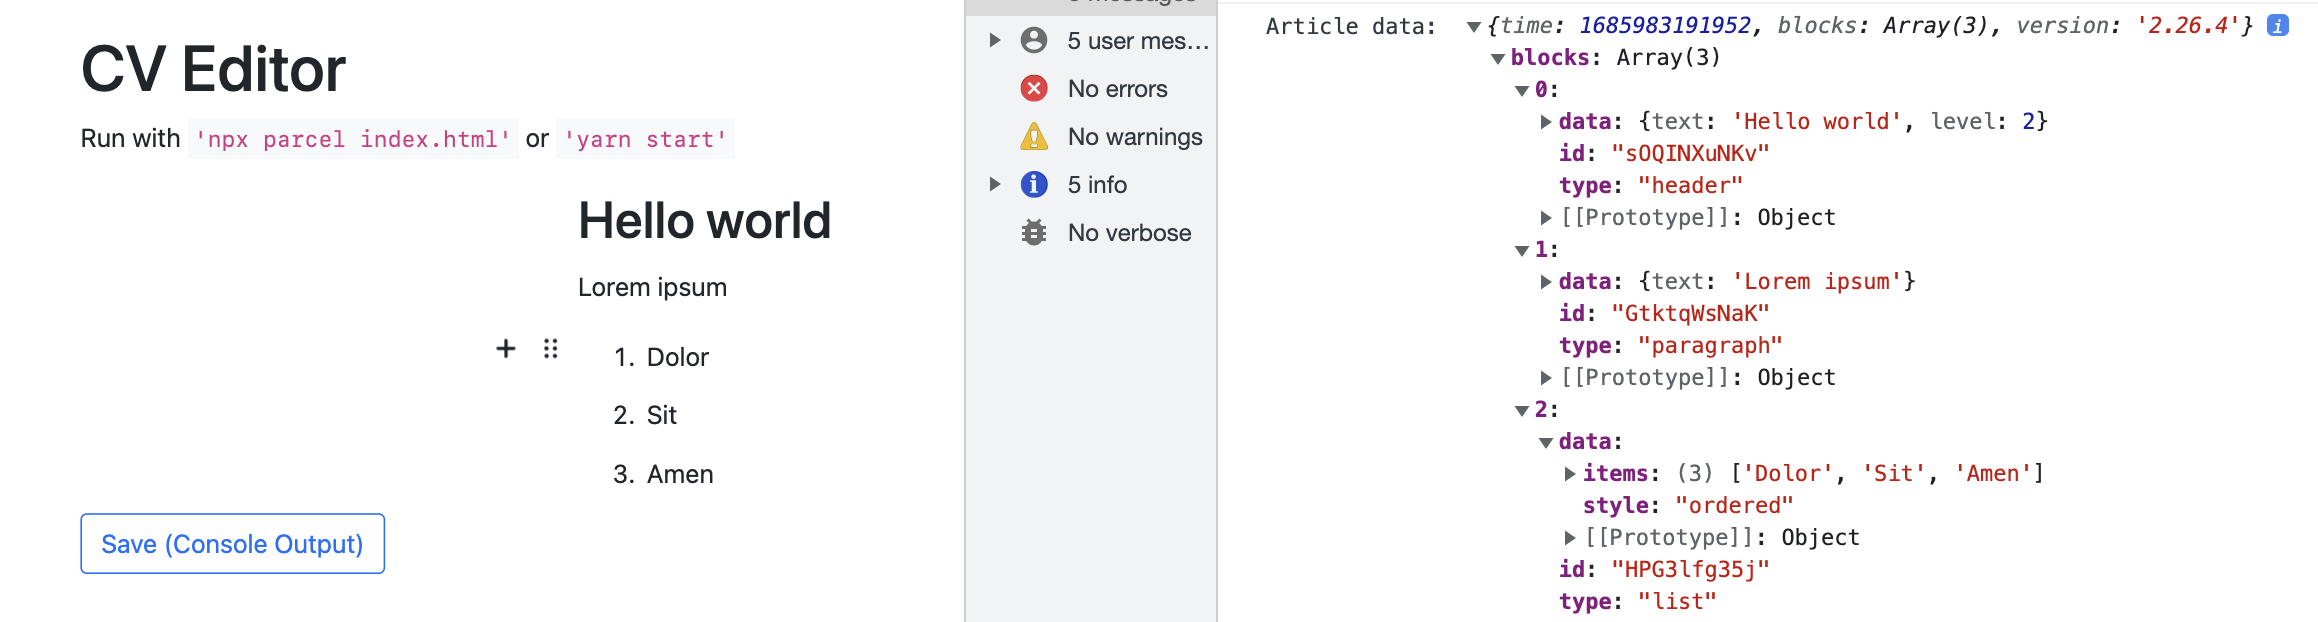
\includegraphics[width=12cm]{images/image22.png}
    \caption{\label{fig:21}%
        Внешний вид свободного редактора данных}
\end{figure}

Реализуем вкладки для шаблона с двумя экранами: заполненным резюме и полями ввода. Для этого внутрь контейнера добавим список из двух значений, добавим им атрибуты вкладок и обозначим первый таб за активный, чтобы при заходе на страницу платформы бланк загружался сразу.
\begin{minted}[fontsize=\small, breaklines=true, style=bw, linenos]{text}
<div class="container p-4">
    <ul class="nav nav-tabs" id="myTab" role="tablist">
        <li class="nav-item" role="presentation">
        <button class="nav-link active" id="home-tab" data-bs-toggle="tab" data-bs-target="#home" type="button" role="tab" aria-controls="home" aria-selected="true">CV Template</button>
\end{minted}

Согласно дизайну сверстаем шаблон и предусмотрим адаптивное отображение страницы, чтобы сайт корректно показывался как на смартфонах, так и на планшетах и компьюетрах. Для этого необходимо правильно описать стили в классах тегов – от наименьшего или стандартного разрешения к самому большому. 
\begin{minted}[fontsize=\small, breaklines=true, style=bw, linenos]{text}
<h5 class="h5 text-uppercase text-secondary mt-5">
<strong>Персональная информация</strong></h5>
<div class="row">
    <div class="col-6 col-lg-3">Пол</div>
    <div class="col-6 col-lg-3 text-end">Муж</div>
</div>
<div class="row">
    <div class="col-6 col-lg-3">Язык</div>
    <div class="col-6 col-lg-3 text-end">Русский</div>
</div>
\end{minted}

Дополнительно для удобства вёрстки воспользуемся сеткой, представляющей из себя вертикальные направляющие, делящие html-страницу на равные части относительно центра страницы с равными отступами от краёв экрана и равным отступом между колонками. Так на компьютерах с разрешением 1920 пикселей боковой отступ будет составлять 365 пикселей, размер рабочего контейнера – 1190 пикселей, всего будет 12 колонок с расстонием между ними в 30 пикселей. Помимо этого внутренние контейнеры также адаптивно делятся в своих пропорциях, образуя сетку в сетке. Итоговый вид шаблона и первой вкладки показан на рисунке~\ref{fig:22}.
\begin{figure}[!ht]
    \centering
    
\includegraphics[width=12cm]{images/image23.png}
    \caption{\label{fig:22}%
        Отображение вкладки переключения и шаблона}
\end{figure}

После вёрстки бланка резюме необходимо реализовать ручные поля ввода, из которых будет приходить информация для страницы. Разобьём их по категориям и представим пользователю в доступном виде, необходимом для последовательного заполнения. Для этого воспользуемся оформлением стилей из библиотеки Bootstrap и реализуем однострочные, многострочные поля ввода и селекторы, в которых изначально предложены варианты выбора данных и стандартное значение.
\begin{minted}[fontsize=\small, breaklines=true, style=bw, linenos]{text}
<h3 class="h3 pb-2">Personal information</h3>
    <div class="row g-4 pb-4">
        <div class="col-md">
            <div class="form-floating">
                <select class="form-select" id="floatingSelectGrid">
                    <option selected>Select</option>
                    <option value="1">Male</option>
                    <option value="2">Female</option>
                </select>
                <label for="floatingSelectGrid">Gender</label>
            </div>
        </div>
\end{minted}

Результатом написания данного блока является вкладка с множеством полей ввода, показанных на рисунке~\ref{fig:23}.
\begin{figure}[!ht]
    \centering
    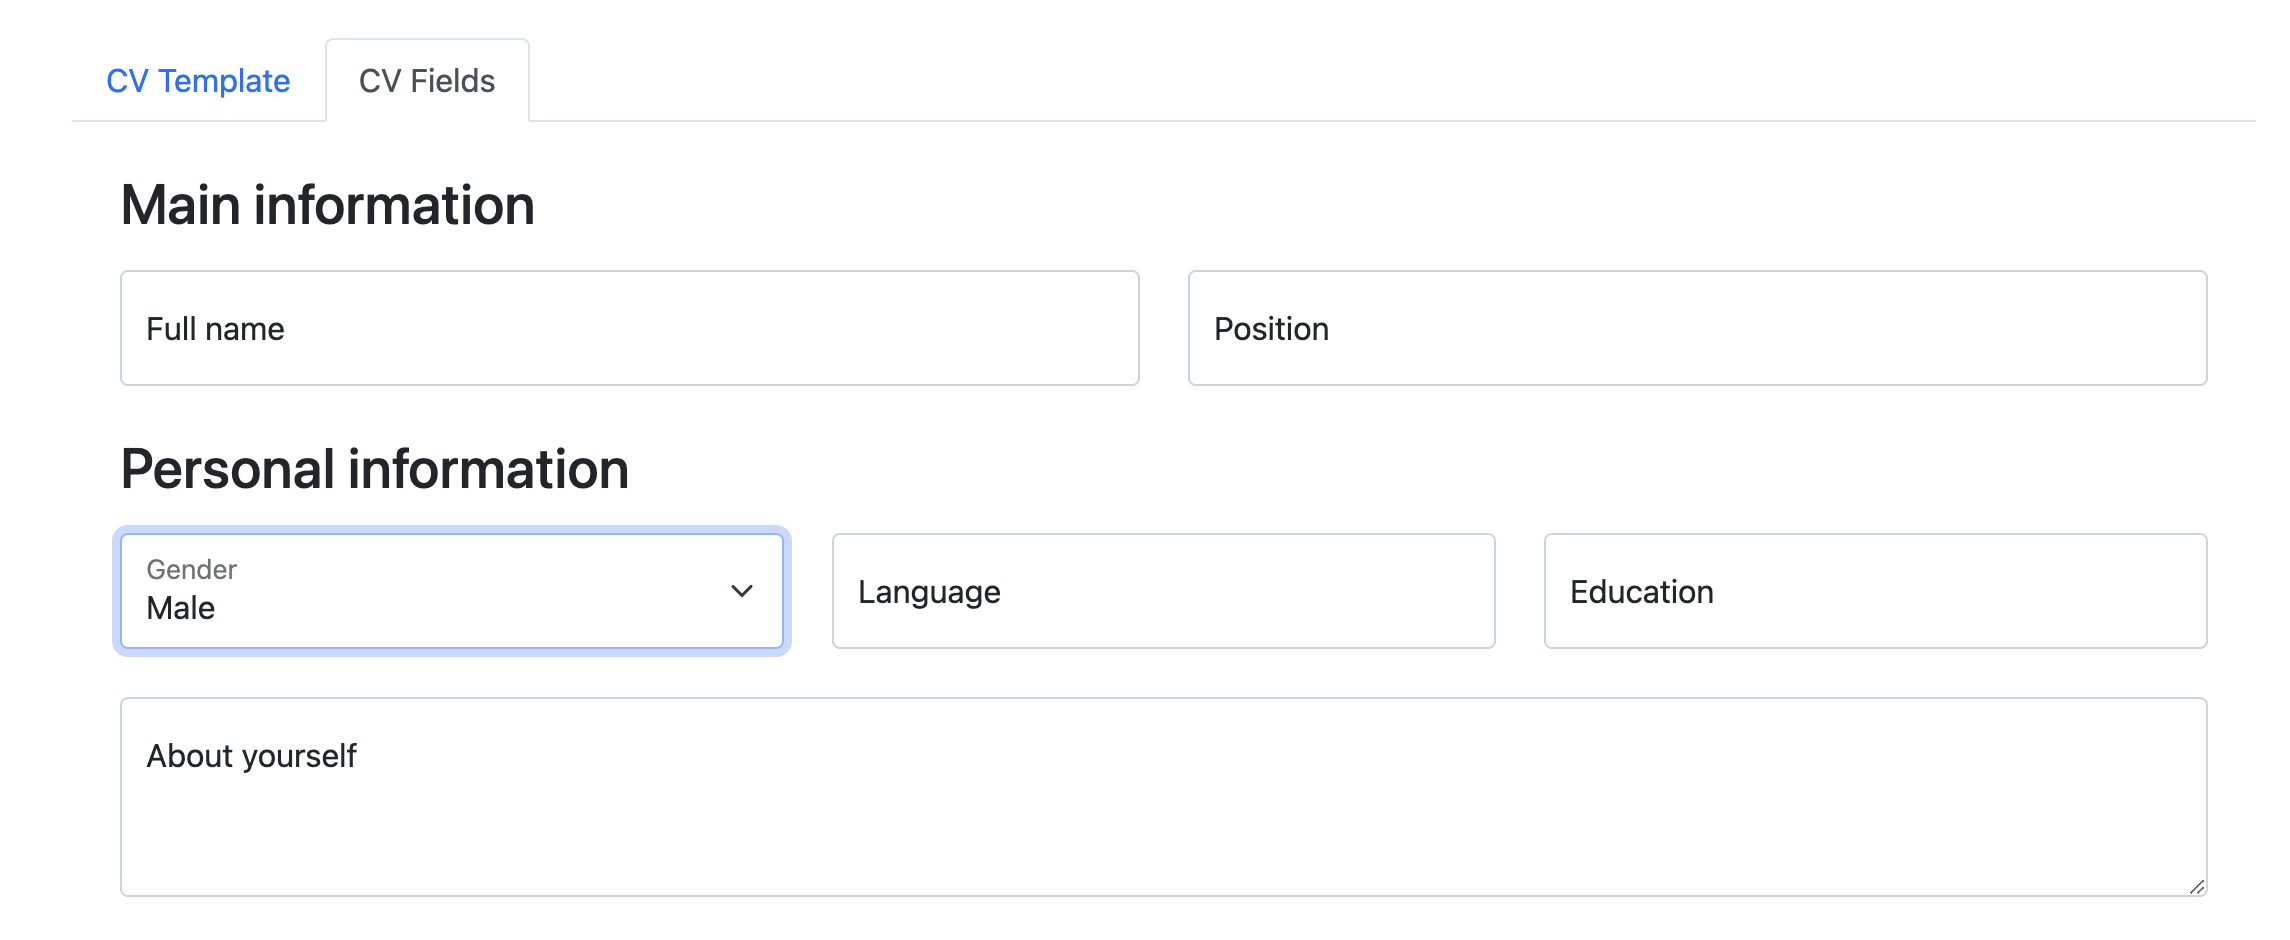
\includegraphics[width=12cm]{images/image24.png}
    \caption{\label{fig:23}%
        Отображение вкладки ввода данных}
\end{figure}

Структура хранения данных о пользователе представляет из себя json-файл, содержащий все описанные выше поля, вроде имени, даты рождения, пола и так далее. Данный выбор формата универсален в рамках нашего приложения и позволяет взаимодействовать с информацией быстрым и удобным способом.
\begin{minted}[fontsize=\small, breaklines=true, style=bw, linenos]{text}
"last_name": "Константинопольский",
"first_name": "Константин",
"middle_name": "none",
"age": 33,
"birth_date": "1991-04-30",
"gender": "male",
\end{minted}



\subsection{Реализация серверной части платформы}
После написания клиентской части приложения необходимо реализовать часть, отвечающую за перенос резюме из сторонних проектов. Для решения поставленной задачи воспользуемся парсером html-страницы на основе библиотеки Puppeteer. Инициируем новый проект аналогично тому, что было в реализации клиентской части и добавим библиотеку для скраппинга:
\begin{minted}[fontsize=\small, breaklines=true, style=bw, linenos]{text}
mkdir parser-cv-editor
cd parser-cv-editor
npm init
yarn add puppeteer
\end{minted}

Работа парсера заключается в создании экземпляра браузера и выполнении заранее прописанных действий. Для этого создадим файл browser.js и опишем логику работы компонента. Так как браузер будет открываться в терминальном состоянии – его визуальное представление необходимо только для отладки работы и во время публикации параметр можно выключить:
\begin{minted}[fontsize=\small, breaklines=true, style=bw, linenos]{text}
const puppeteer = require('puppeteer');
async function startBrowser(){
	let browser;
	try {
	    console.log("Opening the browser");
	    browser = await puppeteer.launch({
	        headless: true,
	        args: ["--disable-setuid-sandbox"],
	        'ignoreHTTPSErrors': true
	    });
	} catch (err) {
	    console.log("Could not create a browser instance => : ", err);
	}
	return browser;
}
module.exports = {
	startBrowser
};
\end{minted}

За управлением экземпляра браузера отвечает pageController.js. В его задачи входит проход по указанной странице и сохранение полученных данных в хранилище в формате json. Для этого подключается с помощью require в Node JS подключается работа с файловой системой, после чего инициализируется объект браузера и через асинхронную функцию происходит считывание страницы с её последующей записью. Дополнительно реализуем обработчик исключений чтобы работа серверной части не нарушалась в случае возникновения ошибок как в момент перехода на страницу, так и в момент записи информации:
\begin{minted}[fontsize=\small, breaklines=true, style=bw, linenos]{text}
const fs = require('fs');
async function scrapeAll(browserInstance){
    let browser;
	try{
	    browser = await browserInstance;
	    let scrapedData = {};
	    scrapedData = await pageScraper.scraper(browser);
	    fs.writeFile("data.json", JSON.stringify(scrapedData), 'utf8', function(err) {
		    if(err) {return console.log(err);}
		    console.log("Done");
	    });
    } catch(err){console.log("Error in ", err);}
}
module.exports = (browserInstance) => scrapeAll(browserInstance)
\end{minted}

После описания вспомогательных файлов серверной части платформы необходимо реализовать точку входа в приложение. Для этого в index.js подключим вышеописанные компоненты, создадим экземпляр браузера и запустим работу контроллера с данным объектом:
\begin{minted}[fontsize=\small, breaklines=true, style=bw, linenos]{text}
const browserObject = require('./browser');
const scraperController = require('./pageController');
let browserInstance = browserObject.startBrowser();
scraperController(browserInstance)
\end{minted}



\subsection{Написание механизма авторизации}
Для реализации авторизации создадим файл auth.ts, в котором укажем конфигурацию с сервисом Github посредством открытого протокола безопасности OAuth и с классической проверкой логина и пароля. Для этого создадим два соответсвующих свойства и в первое передадим переменные приложения для авторизации через сторонний сервис, а в втором реализуем проверку введённых в поля данных и в случае соответсвия вернём самого пользователя с его именем, фотографией профиля и ролью\cite{Fain_2022}.
\begin{minted}[fontsize=\small, breaklines=true, style=bw, linenos]{text}
export const authConfig: AuthOptions = { providers: [
    GithubProvider({
        clientId: process.env.GITHUB_ID!,
        clientSecret: process.env.GITHUB_SECRET!,}),
    Credentials({
    credentials: {
        email: { label: 'email', type: 'email', required: true },
        password: { label: 'password', type: 'password', required: true }, },
        async authorize(credentials) {
        if (!credentials?.email || !credentials.password) return null;
        const currentUser = users.find(user => user.email === credentials.email)
        if (currentUser && currentUser.password === credentials.password) {
            const { password, ...userWithoutPass } = currentUser;
            return userWithoutPass as User;}
    return null }})
    ], pages: { signIn: '/signin' } }
\end{minted}

Ограничение доступа неавторизованного пользователя к внутренним и закрытым страницам достигается созданием файла middleware.ts, в котором через параметры указываются пути навигации и, в случае попадания в заданный путь, перевод клиента на страницу signIn.
\begin{minted}[fontsize=\small, breaklines=true, style=bw, linenos]{text}
export const config = { matcher: ['/profile/:path*', '/hh', 
    '/resume','/protected/:path*'] }
\end{minted}

Дополнительно к предыдущему пунту контроля доступа опишем корневой файл providers.tsx, созданный для окружения корневого элемента страницы в её компоненты, свойства стилей и сессию пользователя.
\begin{minted}[fontsize=\small, breaklines=true, style=bw, linenos]{text}
export function Providers({ children, themeProps }: ProvidersProps) {
return (
<SessionProvider><NextUIProvider>
    <NextThemesProvider {...themeProps}>
        {children}
    <NextThemesProvider>
<NextUIProvider><SessionProvider>);}    
\end{minted}

Процесс авторизации реализуется на клентской и серверной части приложения, поэтому для корректного взаимодействия необходимо создать обработчик событий по API в динамическом маршруте [..auth]/route.tsx с следующими параметрами:
\begin{minted}[fontsize=\small, breaklines=true, style=bw, linenos]{text}
const handler = NextAuth(authConfig);
export { handler as GET, handler as POST }
\end{minted}

Реализуем форму авторизации через компонент SignInForm с двумя текстовыми формами, для этого инициализируем роутер переходов, обратные вызовы для динамического контента и обработчик нажатия кнопки отправки формы, получающий данные полей и выполняющий вход в систему.
\begin{minted}[fontsize=\small, breaklines=true, style=bw, linenos]{text}
const SignInForm = () => {
    const router = useRouter();
    const [isVisible, setIsVisible] = React.useState(false);
    const toggleVisibility = () => setIsVisible(!isVisible);
    const handleSubmit: FormEventHandler<HTMLFormElement> = async (event) => {
        event.preventDefault();
        const formData = new FormData(event.currentTarget);
        const res = await signIn("credentials", {
            email: formData.get("email"),
            password: formData.get("password"),
            redirect: false
}}}
\end{minted}

Кнопка авторизации через Github работает через параметры поисковой строки, получаемые в процессе возврата на страницу платформы после успешного входа на стороне внешнего сервиса.
\begin{minted}[fontsize=\small, breaklines=true, style=bw, linenos]{text}
export const GithubButton = () => {
const searchParams = useSearchParams();
const callbackUrl = searchParams.get("callbackUrl") || "/profile";
return (
    <Button onClick={() => signIn("github", { callbackUrl })}>        
        Log In with GitHub
    </Button>
);};
\end{minted}

После написания компонентов необходимо создать саму страницу авторизации, для этого внутрь всей иерархической оболочки страниицы передадим заголовок вместе с компонентами SignInForm и GithubButton, после которых страница будет располагаться по маршруту app/signIn. Итоговый вид страницы авторизации отображён на рисунке~\ref{fig:24}. 
\begin{figure}[!ht]
    \centering
    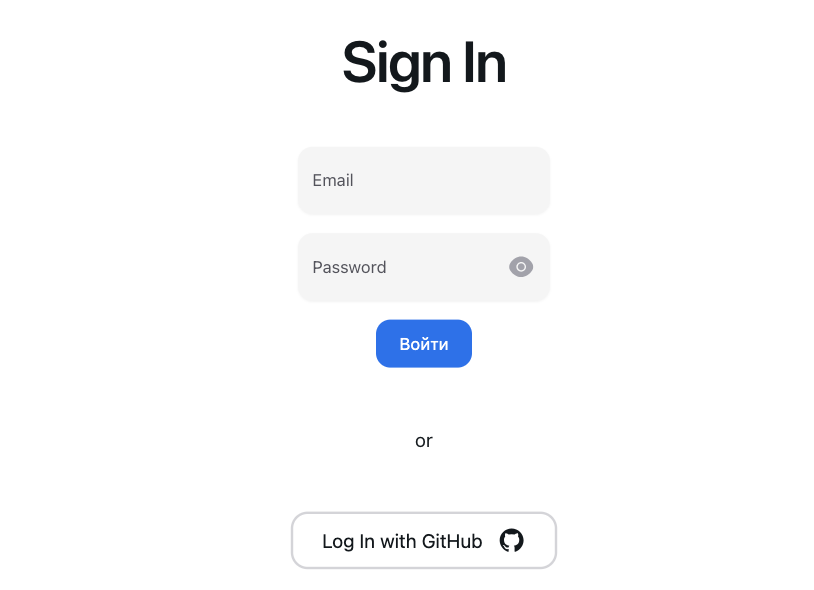
\includegraphics[width=12cm]{images/image-signin.png}
    \caption{\label{fig:24}%
        Страница авторизации}
\end{figure}

Для запуска базы данных на локальном устройстве необходимо воспользоваться средством виртуализации Docker. Скопируем образ из официального репозитория сервиса, запустим из этого образа полноценный контейнер с названием проекта с переадресацией порта на системный 27017 и подключимся к нему из командной строки для проверки работоспособности. Данный порт и адрес потребуются для подключения к базе изнутри сервиса.
\begin{minted}[fontsize=\small, breaklines=true, style=bw, linenos]{text}
docker pull mongodb/mongodb-community-server:latest
docker run --cv-editor mongodb -p 27017:27017 -d mongodb/mongodb-community-server:latest
mongosh --port 27017
\end{minted}

Интегрируем базу данных в механизм авторизации. Для это добавим адаптер MongoDB с помощью следующей команды:
\begin{minted}[fontsize=\small, breaklines=true, style=bw, linenos]{text}
npm install @auth/mongodb-adapter mongodb
\end{minted}

После подключения библиотеки в проект необходимо создать переменную Mongodb-URI в файле process.env с ссылкой на подключение к проекту и в файле auth.ts импортировать необходимые зависимости и инициализировать адаптер в файле авторизации.
\begin{minted}[fontsize=\small, breaklines=true, style=bw, linenos]{text}
import NextAuth from "next-auth";
import { MongoDBAdapter} from "@auth/mongodb-adapter";
import clientPromise from "./lib/db";

export const { handlers, auth, signIn, signOut } = NextAuth({
    adapter: MongoDBAdapter(clientPromise),
});
\end{minted}

После настройки и подключения зависимостей необходимо создать файл взаимодействия с базой данных db.ts и описать соединение. Импортируем клиент и сервер взаимодействия, последовательно получая и проверяя ссылку на подключение с помощью обработчика ошибок. Опишем переменные с включёнными свойствами версии API, его режимом и проверкой целостности.
\begin{minted}[fontsize=\small, breaklines=true, style=bw, linenos]{text}
import { MongoClient, ServerApiVersion } from "mongodb";

if (!process.env.MONGODB_URI) {
    throw new Error('Invalid/Missing environment variable: "MONGODB_URI"');
}
const uri = process.env.MONGODB_URI;
const options = {
    serverApi: {
        version: ServerApiVersion.v1,
        strict: true,
        deprecationErrors: true,
},};
\end{minted}

Создадим синхронного и асинхронного клиента подключения к базе данных и добавим проверку типа запущенного приложения, чтобы в режиме разработки использовать глобавльную переменную окружения для сохранения значения при перезагрузке модуля соединения, вызванных особенностью библиотеки HMR (горячая замена модуля). В зависимости от того, запущен проект на внешнем сервере или на локальном устройстве клиенту присваивается описанная ранее ссылка с переданными свойствами и производится подключение к базе данных. Полный код реализации компонента подключения к базе данных можно найти в приложении А.
\begin{minted}[fontsize=\small, breaklines=true, style=bw, linenos]{text}
let client; let clientPromise: Promise<MongoClient>;
 
if (process.env.NODE_ENV === "development") {
    let globalWithMongo = global as typeof globalThis & {
        _mongoClientPromise?: Promise<MongoClient>
    };
    if (!globalWithMongo._mongoClientPromise) {
        client = new MongoClient(uri, options);
        globalWithMongo._mongoClientPromise = client.connect();
    }
    clientPromise = globalWithMongo._mongoClientPromise;
} else {
    client = new MongoClient(uri, options);
    clientPromise = client.connect();
};
export default clientPromise;
\end{minted}



\subsection{Реализация страницы резюме}
Для написания модуля необходимо создать структуру данных резюме. Информация о профиле хранится в текстовом формате обмена данными JSON и содержит в себе следующие поля:
\begin{enumerate}
    \item Id -- генерируемый уникальный идентификатор резюме;
    \item Name -- фамилия и имя человека;
    \item Description -- краткое описание профиля;
    \item Social links -- ссылки на социальные сети;
    \item Profile image -- изображение работника для резюме;
    \item About -- текстовое поле с рассказом о себе, являющееся аналогом сопроводительного письма;
    \item Education, experience -- группы образования и опыта работы, включающие в себя следующие пункты:
    \begin{enumerate}
        \item Name -- наименование места работы или учебного учереждения;
        \item Description -- описание чем занимался соискатель в данное время;
        \item Start date, end date -- дата начала и окончания; 
        \item Current date -- поле, показывающее что дата окончания отсутвует и при подсчёте её следует считать текущим днём;
    \end{enumerate}
    \item Projects -- поле проектов, следующее из опыта работы. Включает в себя:
    \begin{enumerate}
        \item Name -- наименование проекта;
        \item Description -- описание проекта и над чем происходила работа;
        \item Image -- изображение проекта, его логотип, интерфейс.
    \end{enumerate}
\end{enumerate}

Последовательно реализуем компоненты, начиная с блока контактов и ссылок на социальные сети, получающий на вход список адресов и возвращающий горизонтальный список кнопок с переходом и миниатюрами соответвующих сервисов. Изображения предварительно описываются в формате svg в компоненте icons.tsx, после чего из строки выделяется имя хостинга с последующим добавлением в массив элементов для отображения на странице.
\begin{minted}[fontsize=\small, breaklines=true, style=bw, linenos]{text}
function IconVariant(service: string, icon_color:string, icon_size:number) {
switch(service) { 
    case "github.com": 
        { return <GithubIcon className={icon_color} size={icon_size}/>; } 
    default: 
        { return <InternetIcon className={icon_color} size={icon_size}/>; }
}};
export const SocialLink = (props : SocialProps) => {
    const icon_size, icon_color = 36, "text-default-500";
    const social_icons = props.links.map((element, index) => {
    var url = new URL(element.toString());
return 	
    <Link isExternal href={element.toString()} key={index}>
        {IconVariant(url.host.toString(), icon_color, icon_size)}
    </Link>;
});};
\end{minted}

Итоговый вид компонента показан на рисунке~\ref{fig:25}. 
\begin{figure}[!ht]
    \centering
    
\includegraphics[width=12cm]{images/image-resume-1.png}
    \caption{\label{fig:25}%
        Компонент отображения контактов и ссылок}
\end{figure}

Опишем компонент вывода образования и опыта работы. Для этого реализуем функционал подсчёта текущего затраченного времени через получение двух строковых и одной логической переменных из файла резюме, преобразования текста в объект даты и нахождения разницы между двумя величинами. После вычисления необходимо округлить полученное значение до целого числа и преобразовать в удобочитаемый внешний вид с помощью проверки количества месяцев и лет. Результатом работы функций станет вывод временного значения в строке компонента. Полный код реализации компонента можно найти в приложении Б.
\begin{minted}[fontsize=\small, breaklines=true, style=bw, linenos]{text}
function diffDates(day_one:any, day_two:any) {
    return (day_one - day_two) / (60 * 60 * 24 * 1000);
};
function getFormatedStringFromDays(numberOfDays:number) {
    var months = Math.floor(numberOfDays % 365 / 30);
    var yearsDisplay = years > 0 ? 
        years + (years == 1 ? " year " : " years ") : "";
    return yearsDisplay + monthsDisplay; 
};
export const Experience = (props : ExperienceProps) => {
const experience_item_list = props.experience_list.map((element, index)=>{
    return { getFormatedStringFromDays(diffDates(element.start_date, element.end_date))}})
return  <>{experience_item_list}</>
};
\end{minted}

Итоговый вид компонента показан на рисунке~\ref{fig:26}.  
\begin{figure}[!ht]
    \centering
    
\includegraphics[width=12cm]{images/image-resume-2.png}
    \caption{\label{fig:26}%
        Компонент отображения опыта работы и образования}
\end{figure}

Для реализации портфолио в шахматном представлении воспользуемся классовыми атрибутами сетки из библиотеки Tailwind. Получим порядковый индекс списка проектов, начинающийся с нуля, и дальше в зависимости от чётности раздельно и поочерёдно позиционируем текст с 1 по 6 колонку и изображение с 7 по 13.
\begin{minted}[fontsize=\small, breaklines=true, style=bw, linenos]{text}
export const Projects = (props : ProjectsProps) => {
const projects = props.projects_list.map((element, index) => {
    var position_image = index % 2 == 0 ? 
        "col-start-7 col-end-13" : "col-start-1 col-span-6 ";
    var position_text = index % 2 == 0 ? 
        "col-start-1 col-end-6" : "col-start-8 col-end-13 order-1";
    return (
        <div className={position_text}>
            <h2>{element.name}</h2>
            <p>{element.description}</p>
        </div>
        <Image className={position_image}/>
    )})
return <>{projects}</>
};
\end{minted}

Итоговый вид компонента списка проектов показан на рисунке~\ref{fig:27}. 
\begin{figure}[!ht]
    \centering
    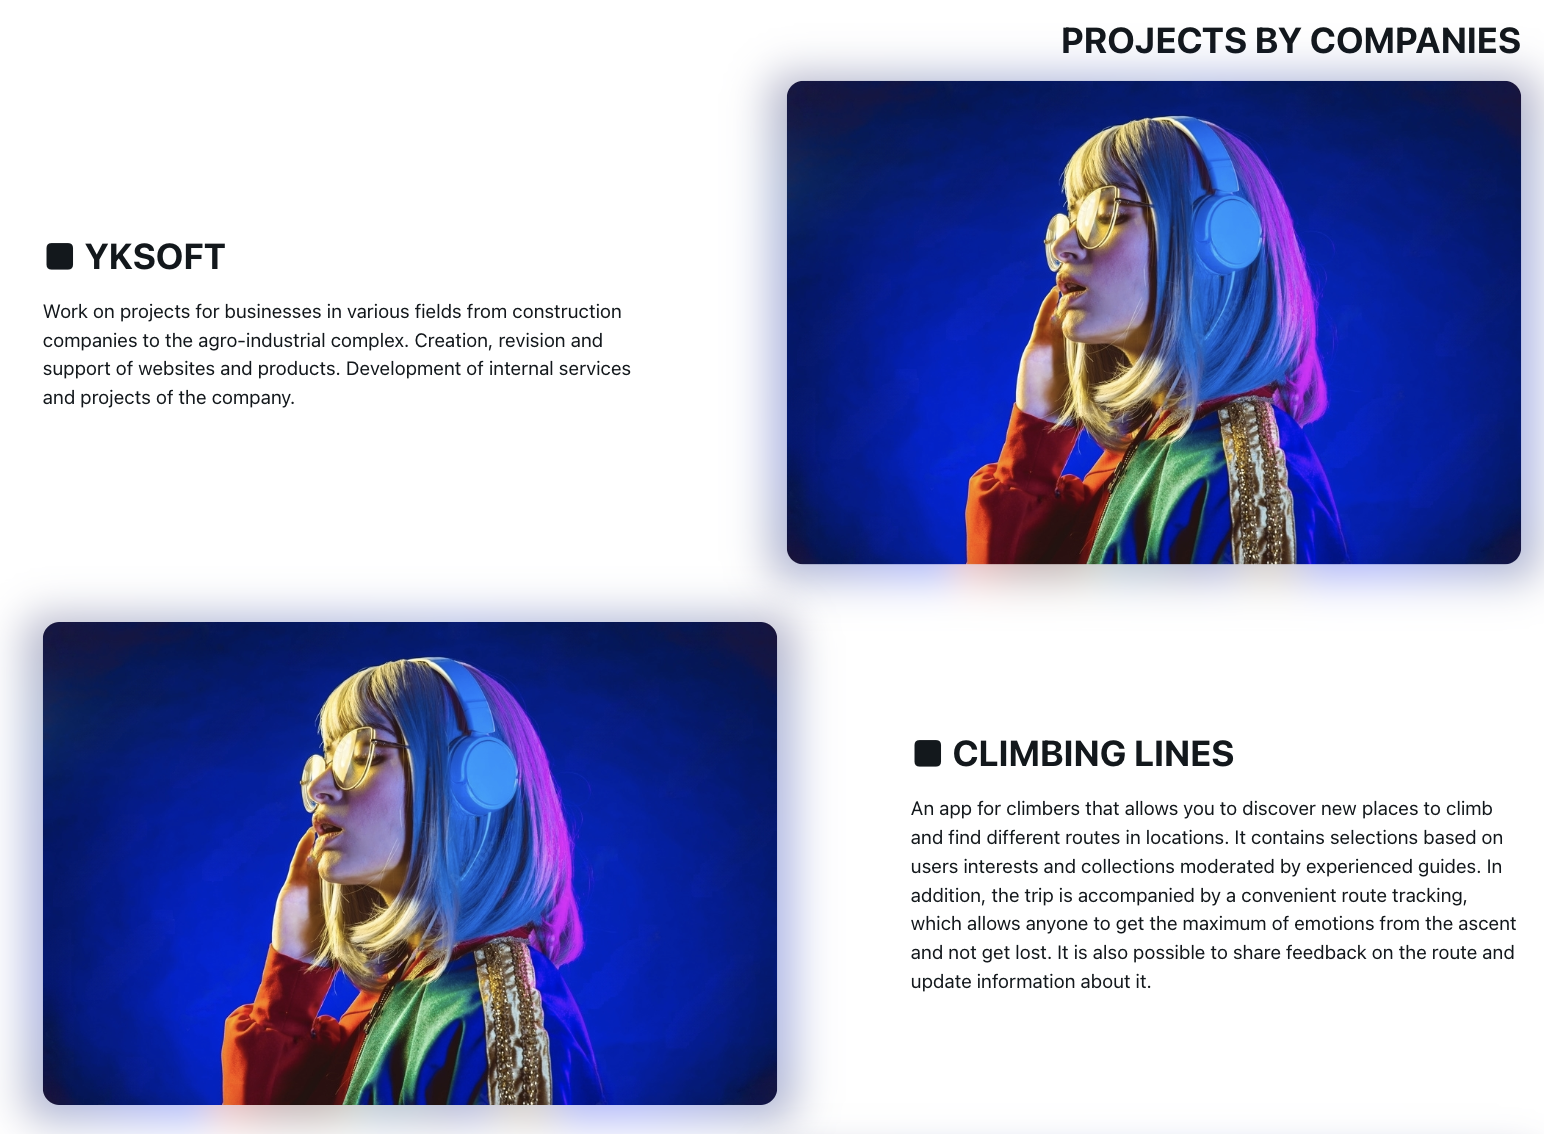
\includegraphics[width=12cm]{images/image-resume-3.png}
    \caption{\label{fig:27}%
        Компонент отображения списка проектов}
\end{figure}

После описания компонентов реализуем страницу резюме, для этого необходимо произвести запрос данных резюме и передать его поля в соответвующие теги и компоненты. Полный код реализации страницы можно найти в приложении В.  
\begin{minted}[fontsize=\small, breaklines=true, style=bw, linenos]{text}
export default function Template1Page() {
const profile_data = require("@/data-template/template-1-data.json");
return (
<SocialLink links = {profile_data.social_links}/>
<div className="container pt-5 pb-5">
    <h2 id="projects">projects by companies</h2>
    <Projects projects_list={...profile_data.projects}/></div>);}    
\end{minted}



\subsection{Взаимодействие с сервисом hh.ru}
Реализуем взаимодействие пользователя с сервисом hh.ru через API. Первоначальная конфигурация в виде авторизации состоит из 3 этапов:
\begin{enumerate}
    \item Перенаправление пользователя по адресу сервиса с переданными параметрами строки;
    \item Получение временного кода авторизации;
    \item Обмен кода авторизации на долгосрочный токен доступа к профилю и кода обновления токена в случае необходимости.\cite{hh_api}
\end{enumerate}

Первый этап достигается с помощью передачи параметров строки запроса через вопросительный знак, имя параметра и значение. В ответ на полученную от сервиса hh.ru ссылку с переходом необходимо обработать ответный параметр временного кода авторизации и обмена на долгосрочный. Опишем данный функционал в api/hh/route.tsx, для этого необходимо реализовать GET запрос, предварительно считывающий строку запроса и параметр code, в заголовок которого добавляем желаемое действие, открытый и секретный идентификаторы приложения и полученный на предыдущем обработчике код. Так как функция запросов асинхронна – воспользуемся обработчиком событий и через ожидающий асинхронный обратный вызов функции передадим запрос по адресу сервиса, получив в ответ необходимый набор данных: ответ об успешности запроса и токены\cite{Razin_2020}.
\begin{minted}[fontsize=\small, breaklines=true, style=bw, linenos]{text}
export async function GET(req: Request) {
const { searchParams } = new URL(req.url)
const code = searchParams.get('code');
if (code != null) {
    myHeaders.append("Content-Type", "application/x-www-form-urlencoded");
    urlencoded.append("grant_type", "authorization_code");
    urlencoded.append("client_id", process.env.HH_ID!);
    urlencoded.append("client_secret", process.env.HH_SECRET!);
    urlencoded.append("code", code!);
    try {
        const res = await fetch("https://hh.ru/oauth/token", {
            method: 'POST', headers: myHeaders,
            body: urlencoded, redirect: 'follow' });   
        const result = await res.json();
        return NextResponse.json(result);
}} 
\end{minted}

После получения долгосрочного токена для конкретного пользователя, у приложения появляется возможность воспользоваться доступом к сервису hh.ru. Получим все существующие резюме человека и выведем их на страницу. Для этого отправим GET запрос с токеном авторизации по заданному маршруту и вернём данные в формате JSON.
\begin{minted}[fontsize=\small, breaklines=true, style=bw, linenos]{text}
const token = searchParams.get('token');
if (token != null) {
    var myHeaders = new Headers();
    myHeaders.append("Authorization", `Bearer ${token}`);
    try {
        const res = await fetch("https://api.hh.ru/resumes/mine", {
            method: 'GET', headers: myHeaders, redirect: 'follow' });      
        const result = await res.json();
        return NextResponse.json(result);
}}
\end{minted}



\subsection{Реализация страниц сравнения и обновления резюме}
Страница сравнения навыков представляет из себя таблицу, содержащую наименование поля, значения совпадающих ключей для каждого из входных резюме и поле взаимодействия, содержащее возможность добавления собственного значения, а также удаления строки. Так как резюме содержит в себе значениях разных типов, их отображение будет возможно только при разделениии. Для этого реализуем компонент сравнения, получающий значение свойства из JSON и далее в случае одиночной строки возвращающий тег с его содержимым, в случае списка строк обрабатывающий каждую из них, присваивающую уникальный индекс отображения, а в случае более глубокой вложенности добавляющей перед элементом его наименование.
\begin{minted}[fontsize=\small, breaklines=true, style=bw, linenos]{text}
if (typeof props.cv_editor == "string") {
    cv_editor_item_list = <div>{props.cv_editor}</div>;
} else {
    Object.keys(props.cv_editor).map((element, index) => {
    let arrObj = props.cv_editor[element];
    if (typeof arrObj == "object") {
    cv_editor_item_list = props.cv_editor.map((element: any, index:any) => {
    return (
        {Object.keys(element).map((el, index) => {
        return( <div key={index}>{el}: {element[el]}</div> );})}
    );});  
    } else {
        cv_editor_item_list = props.cv_editor.map((element: any, index:any) => 
        { return {element}; })
}});}
\end{minted}

Итоговый вид страницы сравнения навыков показан на рисунке~\ref{fig:28}. 
\begin{figure}[!ht]
    \centering
    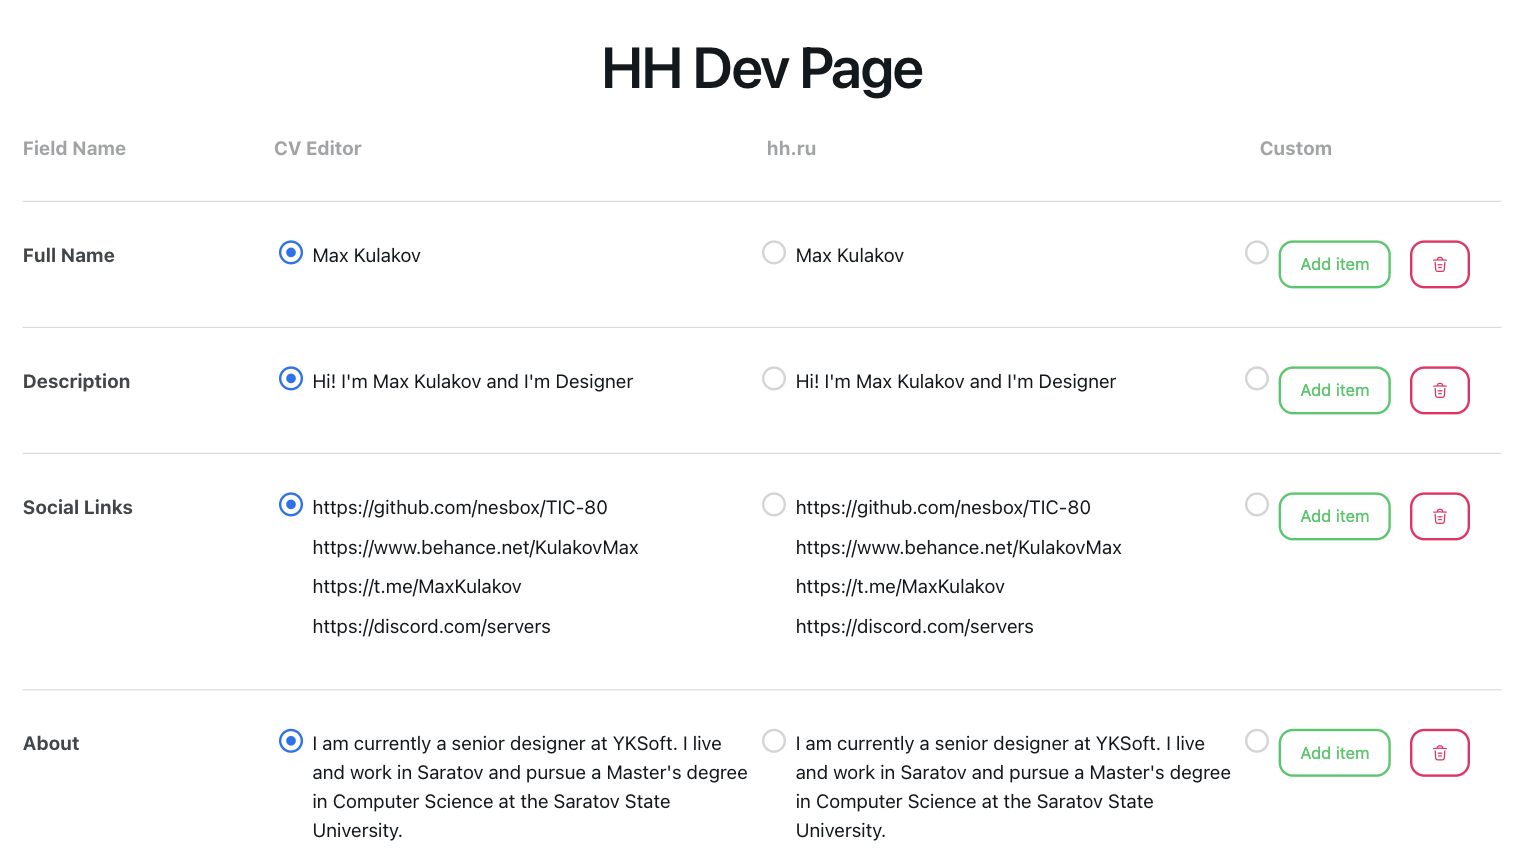
\includegraphics[width=12cm]{images/image-compare-skills.png}
    \caption{\label{fig:28}%
        Страница сравнения навыков}
\end{figure}

В серверной части платформы реализуем API метод для обновления данных резюме на сервисе hh.ru. Для этого в файле api/hh/route.tsx опишем PUT запрос, в заголовок которого передаётся токен пользователя и ссылка на идентификатор резюме, а в тело наименование поля данных с его содержимым. После выполнения запроса в ответ от внутреннего сервера вернётся JSON с кодом и сообщением об успешности выполненной операции.
\begin{minted}[fontsize=\small, breaklines=true, style=bw, linenos]{text}
export async function PUT(req: Request) {
if (resume != null) {
    const body = await req.json()      
    var raw = JSON.stringify( body );
    try { const res = await fetch(`https://api.hh.ru/resumes/${resume}`,{
        method: 'PUT', headers: myHeaders,
        body: raw, redirect: 'follow' })
    return NextResponse.json({ message: "Resume has been updated" });
}}}
\end{minted}

Реализуем страницу обновления навыков, для которой запросим и выведем данные из резюме hh.ru в виде списка тегов с возможностью их удаления из списка. Для этого создадим страницу и инициализируем начальное состояние значений и функцию удаления, проверяющую количество элементов и в случае их полного удаления возвращающего к исходному значению.
\begin{minted}[fontsize=\small, breaklines=true, style=bw, linenos]{text}
export default function ResumePage() {
    const [skill_set, setSkill_set] = React.useState(initialSkills);
    const handleClose = (skillToRemove:any) => {
        setSkill_set(skill_set.filter((skill: any) => 
            skill !== skillToRemove));
        if (skill_set.length === 1) {setSkill_set(initialSkills);}
}};
\end{minted}

Добавим кнопку обновления резюме, по нажатию на которую вызывается функция-обработчик массива строк с преобразованием их к объектному формату JSON и помещающая итоговое значение в тело PUT запроса, отправляющего сообщение через внутрненний сервер на сервис hh.ru.
\begin{minted}[fontsize=\small, breaklines=true, style=bw, linenos]{text}
const skills_body = JSON.parse(JSON.stringify
    (`{"skill_set": [${skill_set.map((x: any) => `"${x}"`)}]}`))
return (
skill_set.map((skill: any, index: any) => (
    <Chip key={index} onClose={() => handleClose(skill)} variant="flat">
        {skill}
    </Chip>
    <Button onClick={updateResume}>Обновить резюме</Button>
)))
\end{minted}

Итоговый вид страницы обновления навыков, содержащей статус изменения списка, редактируемое поле ввода и теги представлен на рисунке~\ref{fig:29}. 
\begin{figure}[!ht]
    \centering
    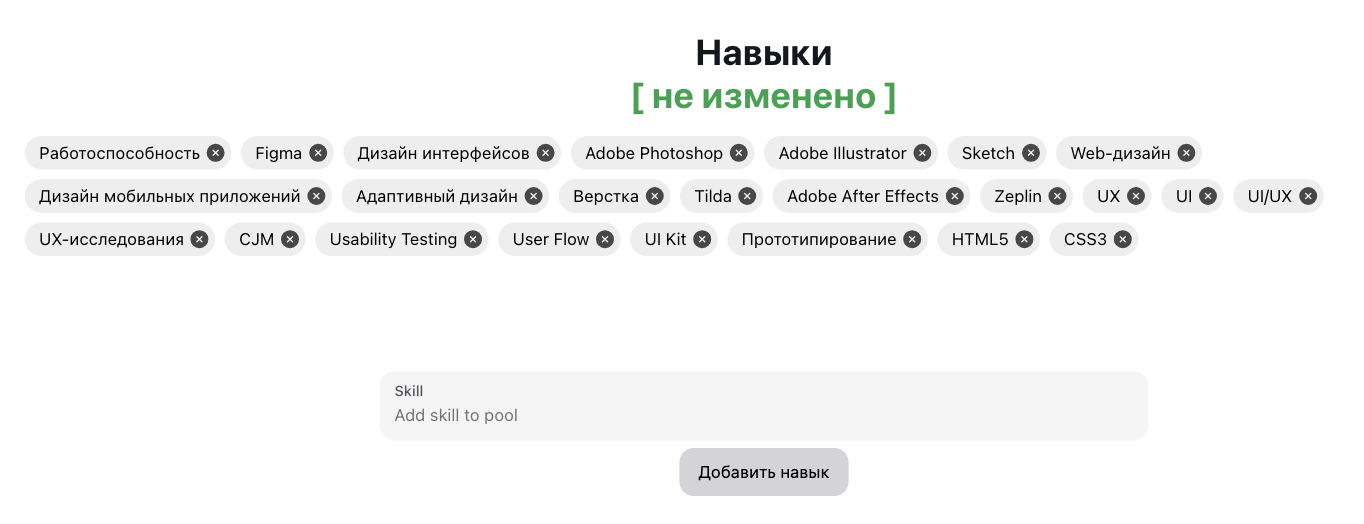
\includegraphics[width=12cm]{images/image-update-skills.png}
    \caption{\label{fig:29}%
        Страница обновления навыков}
\end{figure}



\subsection{Реализация страницы процесса разработки}
Для написания страницы необходимо создать структуру данных в текстовом формате JSON, содержащую в себе следующие поля:
\begin{enumerate}
    \item Type -- тип карточки, делится на работу, находящуюся в процессе и уже выполненную;
    \item Version -- порядковый номер завершённой работы, может принимать отсутствующее значение в случае текущего выполнения, иначе соответсвующее семантическому версионированию, например 1.2.3, где:
    \begin{enumerate}
        \item 1 -- характеризует мажорную версию, в которой происходит значительная переработка поведения, функционала и кода, зачастую с потерей совместимости с предыдущей мажорной версией;
        \item 2 -- соответствует минорной версии, в которой добавляется новый функционал или вносятся изменения в уже существующий проект;
        \item 3 -- является патч версией, включающей исправление ошибок или незначительную переработку кода;
    \end{enumerate} 
    \item Date -- дата публикации выполненной работы;
    \item Task-list -- список звершённых задач, являющийся массивом строк;
    \item Author -- профиль автора, включающий в себя следующие пункты:
    \begin{enumerate}
        \item Thumbnail -- миниатюра профиля;
        \item Name -- имя или псевдоним разработчика;
        \item Team -- команда проекта.
    \end{enumerate} 
\end{enumerate}

Создадим функцию getDate, принимающую дату в международном формате yyyy-mm-dd и преобразующую её в новый объект с типом данных <<Дата>>, обрезанным от лишних для отображения значений дня недели и времени, и читаемым текстовым видом без дефисов.
\begin{minted}[fontsize=\small, breaklines=true, style=bw, linenos]{text}
function getDate(date: string) {
    const temp_date = new Date(date).toUTCString().slice(5, 16);
    return temp_date;
};
\end{minted}

Получим список публикаций и запишем его в константу, предварительно выполнив сортировку по номеру версии. Для этого с помощью стрелочной функции получаем значение у ближайшей пары и сравниваем записанные значения, после чего наименьшее помещаем в конец. Если номера нет и работа находится в процессе, то данный элемент встаёт в начало списка.
\begin{minted}[fontsize=\small, breaklines=true, style=bw, linenos]{text}
const release_list = require("@/data-template/release-data.json").sort(
    (a:any, b:any) => {if (a.version > b.version) { return -1; }}
);
\end{minted}

После этого необходимо отобразить обработанные данные. Для этого создадим контейнер с сеткой, колонками, отступами между блоками и полной шириной, и последовательно передадим в карточку каждого элемента его порядковый номер в списке для унификации компонентов и сами данные.
\begin{minted}[fontsize=\small, breaklines=true, style=bw, linenos]{text}
<div className="gap-4 grid grid-cols-1 sm:grid-cols-4 mt-4 w-full">
    {release_list.map((item:any, index:any) => (...))}
\end{minted}

Опишем компоненты карточки, состоящей из тега Card, шапки карточки, содержащей проверку на тип публикации и в зависимсоти от этого выводящее версию или отображение текущей работы, вместе с соответсвующей датой. После разделителя внутри центральной части карточки идёт перечисление всех задач в списке, и в конце миниатюра с именем и командой автора. Полный код реализации страницы процесса разработки можно найти в приложении Г.
\begin{minted}[fontsize=\small, breaklines=true, style=bw, linenos]{text}
<Card key={index}>
    <CardHeader className="container">
        {item.type == "WIP"?
            <Chip color="primary" variant="bordered">WIP</Chip> : 
            <Chip color="primary" variant="solid">v{item.version}</Chip>}
    </CardHeader><Divider/><CardBody>...</CardBody><Divider/>
    <CardFooter>
        <Image
            isZoomed isBlurred radius="full"
            width={40} height={40}
            src={item.author.thumbnail}/>
        {item.author.name}{item.author.team}
    </CardFooter>
</Card>
\end{minted}

После написания структуры хранения, функций обработки даты и сортировки, вёрстки и стилей, страница принимает вид, представленный на рисунке~\ref{fig:30}.
\begin{figure}[!ht]
    \centering
    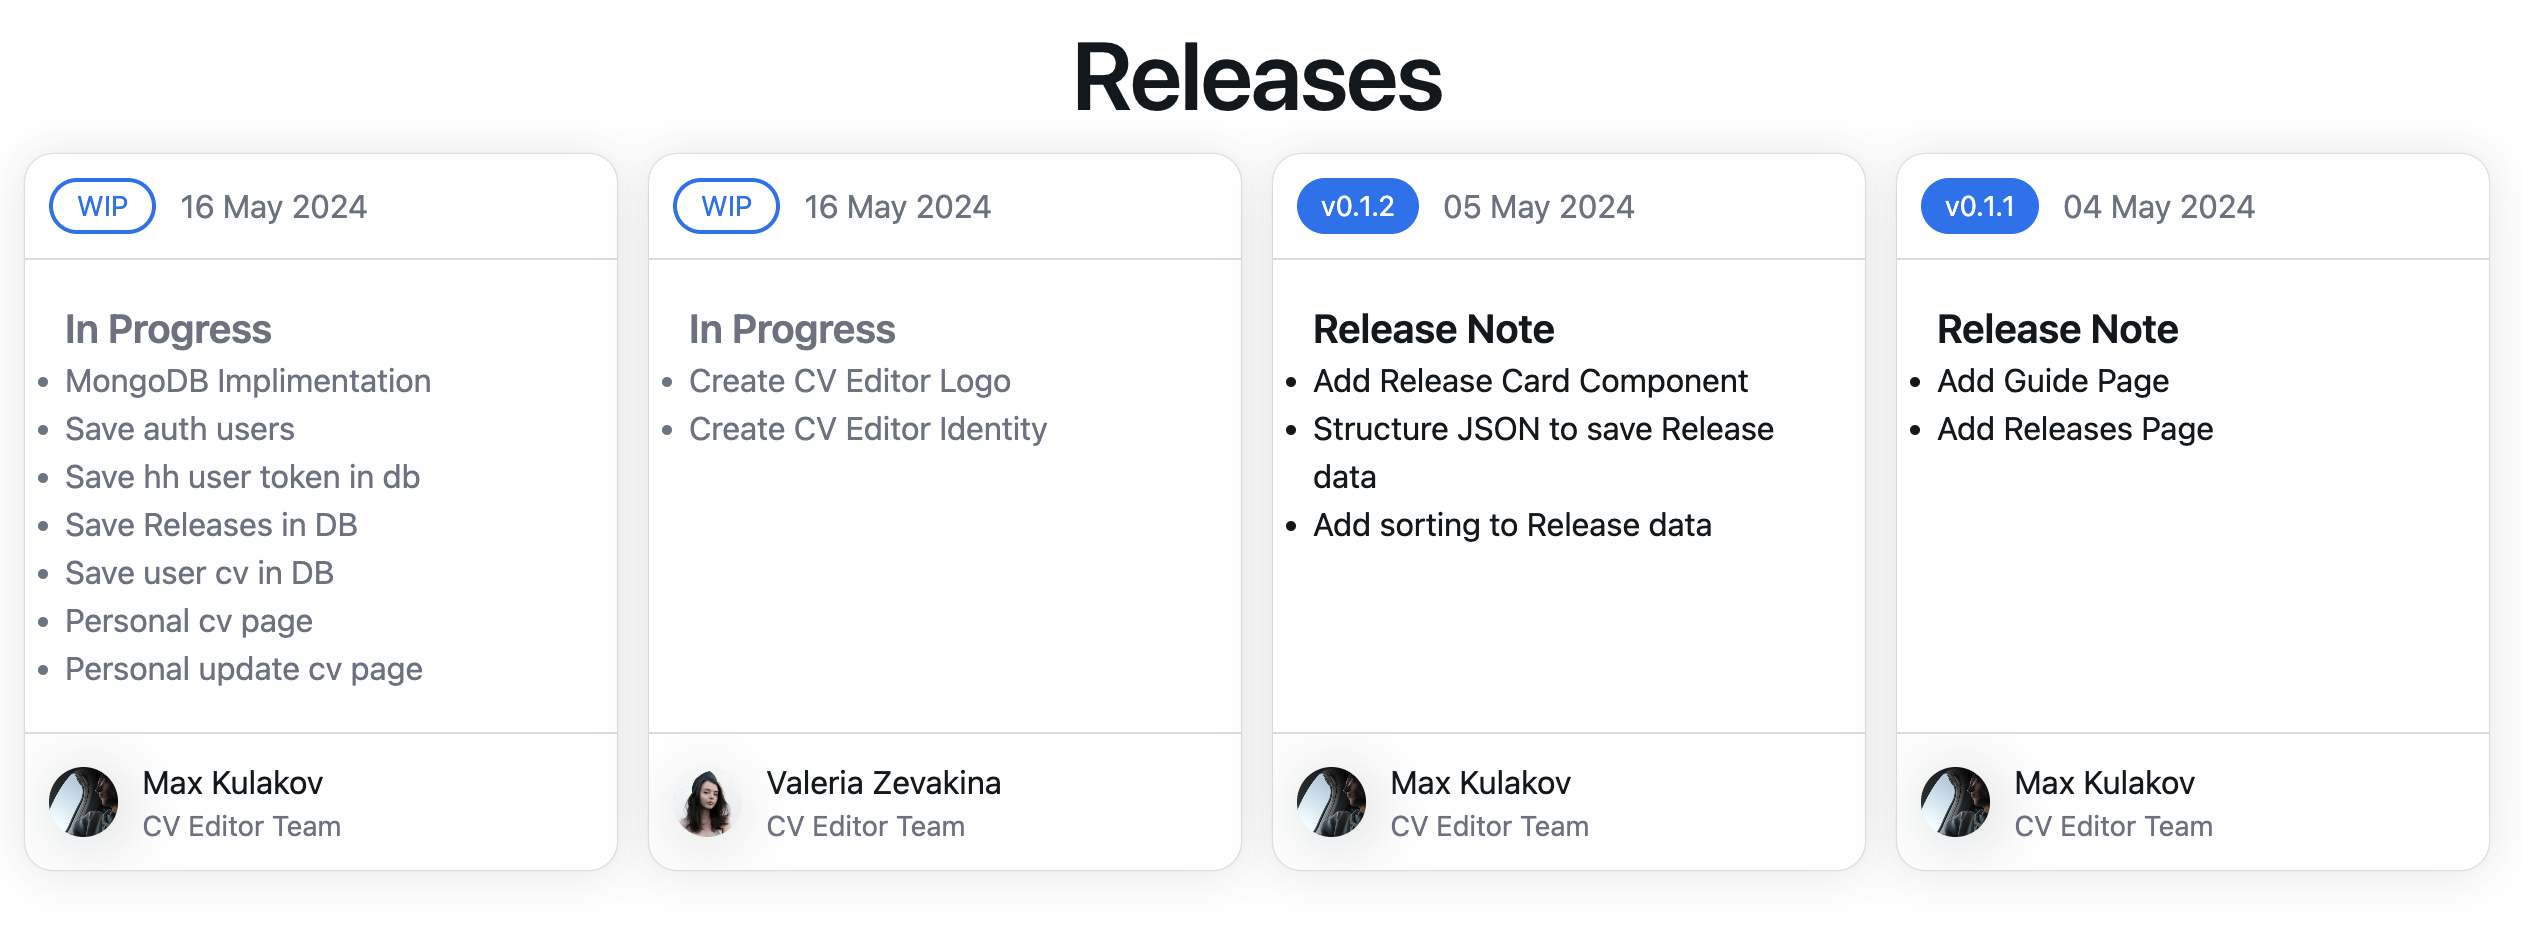
\includegraphics[width=12cm]{images/image-releases.png}
    \caption{\label{fig:30}%
        Страница процесса разработки}
\end{figure} 



\subsection{Публикация платформы единого резюме}
Перед публикацией необходимо изменить файл настроек проекта, указав точку входа и конфигурацию скрипта в файле package.json:
\begin{minted}[fontsize=\small, breaklines=true, style=bw, linenos]{text}
"scripts": {
    "build": "next build",
    "start": "next start"
},
\end{minted}

Так как платформа работает в режиме сервера – публикация в виде статичной страницы не представляется возможным, поэтому воспользуемся хостингом Vercel, позволяющим реализовать данную потребность. Первоначально необходимо загрузить свой код в систему контроля версий GitHub, после чего связать аккаунт с аккаунтом хостинга, синхронизировать репозитории и настроить параметры публикации. В итоговом виде платформа соберётся в оптимизированный для получения пользователем вид, закэшируется в папке dist и будет выдаваться браузеру при обращении по ссылке. Настройки публикации сайта в Vercel представлены на рисунке~\ref{fig:31}.
\begin{figure}[!ht]
    \centering
    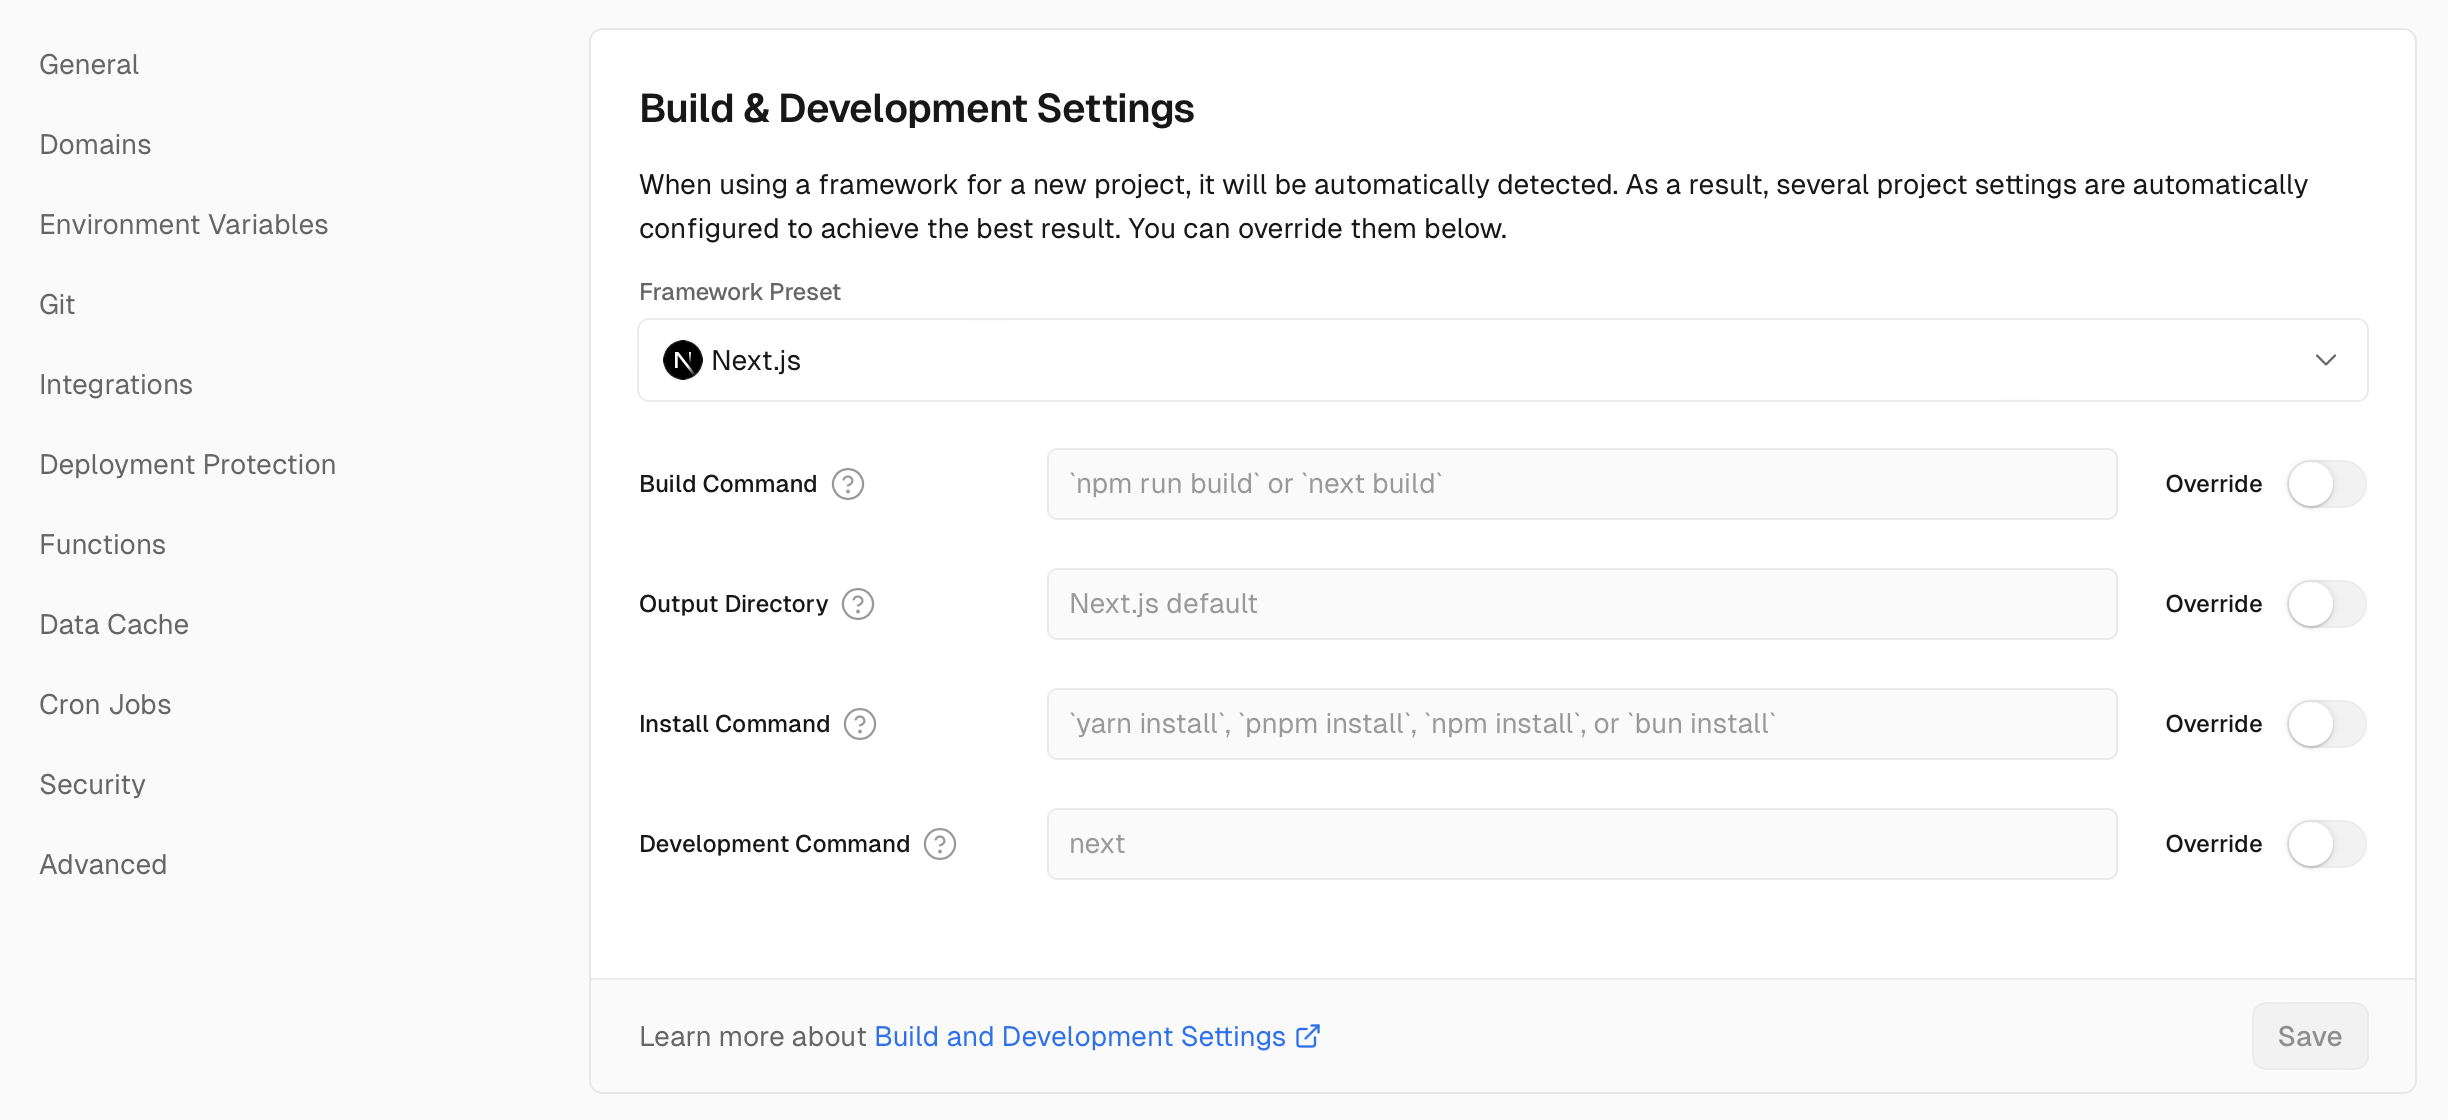
\includegraphics[width=12cm]{images/image-vercel.png}
    \caption{\label{fig:31}%
        Настройка публикации сайта}
\end{figure} 

После написания кода мы получили готовый сервис, в котором реализован весь запланированный функционал: от базовых элементов и компонентов до серверной части с авторизацией и обновлением резюме.






\newpage
\conclusion
В результате проведения исследовательской работы были приобретены навыки анализа качества и эффективности научной литературы в областях веб-разработки, разработки сервисов с автоматическим обновлением данных, а также навык анализирования конкурентных платформ для создания резюме. Анализ статей по составлению резюме, социологическому подходу к этой теме и инструментам веб-разработки позволил сформулировать требования для разработки единой платформы резюме.

Проведенный анализ конкурентных платформ выявил недостатки существующих сервисов, что послужило основой для разработки собственной платформы. Данное решение включает серверную и клиентскую части приложения, а также подразумевает публикацию проекта на серверном хостинге для эффективного взаимодействия с функциональностью платформы.

Результаты данной работы были представлены на студенческой научной конференции факультета КНиИТ в апреле 2024 года.

По итогам выполнения исследовательской работы все поставленные цели и задачи были успешно достигнуты. Были разработаны собственные методы разработки и масштабирования единой платформы резюме. В качестве объектов анализа научной литературы для реализации данного сервиса выступили статьи по темам разработки клиент-серверного приложения средствами библиотек Next JS, TailWind и применением архитектуры Rest API. С учётом проведённого анализа научной литературы были составлены базовые технические требования для масштабирования уже существующего приложения. 






% Библиографический список, составленный вручную, без использования BibTeX
%
% \begin{thebibliography}{99}
%   \bibitem{Ione} Источник 1.
%   \bibitem{Itwo} Источник 2
% \end{thebibliography}

% Отобразить все источники. Даже те, на которые нет ссылок.
% \nocite{*}

% Меняем inputencoding на лету, чтобы работать с библиографией в кодировке
% `cp1251', в то время как остальной документ находится в кодировке `utf8'
\inputencoding{cp1251}
\bibliographystyle{gost780uv}
\bibliography{thesis}
\inputencoding{utf8}

% При использовании biblatex вместо bibtex
% \printbibliography


% Окончание основного документа и начало приложений Каждая последующая секция
% документа будет являться приложением
\appendix

\section{Реализация подключения к MongoDB}
\begin{minted}[fontsize=\small, breaklines=true, style=bw, linenos]{text}
import NextAuth from "next-auth";
import { MongoDBAdapter} from "@auth/mongodb-adapter";
import clientPromise from "./lib/db";
import { MongoClient, ServerApiVersion } from "mongodb";

const { handlers, auth, signIn, signOut } = NextAuth({
    adapter: MongoDBAdapter(clientPromise),
});

if (!process.env.MONGODB_URI) {
    throw new Error('Invalid/Missing environment variable: "MONGODB_URI"');
}

const uri = process.env.MONGODB_URI;
const options = {
    serverApi: {
        version: ServerApiVersion.v1,
        strict: true,
        deprecationErrors: true,
    },
};

let client; let clientPromise: Promise<MongoClient>;
 
if (process.env.NODE_ENV === "development") {
    let globalWithMongo = global as typeof globalThis & {
        _mongoClientPromise?: Promise<MongoClient>
    };
    if (!globalWithMongo._mongoClientPromise) {
        client = new MongoClient(uri, options);
        globalWithMongo._mongoClientPromise = client.connect();
    }
    clientPromise = globalWithMongo._mongoClientPromise;
} else {
    client = new MongoClient(uri, options);
    clientPromise = client.connect();
};

export default clientPromise;
\end{minted}



\section{Реализация компонента отображения опыта}
\begin{minted}[fontsize=\small, breaklines=true, style=bw, linenos]{text}
"use client";
import * as React from "react";

function diffDates(day_one:any, day_two:any) {
    return (day_one - day_two) / (60 * 60 * 24 * 1000);
};

function getFormatedStringFromDays(numberOfDays:number) {
    numberOfDays = Math.abs(numberOfDays)
    var years = Math.floor(numberOfDays / 365);
    var months = Math.floor(numberOfDays % 365 / 30);
    var yearsDisplay = years > 0 ? 
        years + (years == 1 ? " year " : " years ") : "";
    var monthsDisplay = months > 0 ? 
        months + (months == 1 ? " month " : " months ") : "";
    return yearsDisplay + monthsDisplay; 
}

interface ExperienceItemProps {
    name: string;
    description: string;
    start_date: string;
    end_date: string;
    current_date?: boolean;
}

interface ExperienceProps {
    experience_list: ExperienceItemProps[];
}

export const Experience = (props : ExperienceProps) => {
const experience_item_list = props.experience_list.map((element, index) => {
    const date1 = new Date(element.start_date);
    const date2 = element.current_date ? 
        new Date() : new Date(element.end_date)
    
    return (
        <div key={index} className="grid grid-cols-12 gap-2 mb-4">
            <div className="col-start-1 col-end-3">
                {element.start_date} - {element.end_date} 
                <div className="text-default-500">
                    {getFormatedStringFromDays(diffDates(date1, date2))}
                </div>
            </div>
            <div className="col-start-4 col-end-6">
                {element.name}
            </div>
            <div className="col-start-7 col-end-13">
                {element.description} 
            </div>
        </div>
    )
})
return  <>{experience_item_list}</>
};
\end{minted}



\section{Реализация страницы резюме}
\begin{minted}[fontsize=\small, breaklines=true, style=bw, linenos]{text}
"use client";
import React from "react";
import {Image} from "@nextui-org/react";
import { SocialLink } from "@/components/social-link";
import { Experience } from "@/components/experience";
import { Projects } from "@/components/projects";
import { About } from "@/components/about";

export default function Template1Page() {
const profile_data = require("@/data-template/template-1-data.json");
return (
    <h1 className="h6 text-uppercase text-center pb-4">
        {profile_data.name}
    </h1>
    <p className="text-uppercase text-center pb-2">
        {profile_data.description}
    </p>
    <SocialLink links = {profile_data.social_links}/>
    <div className="grid grid-cols-8 gap-4 mb-12">
        <div className="col-start-3 col-end-7">
            <Image
            isZoomed
            isBlurred
            alt={profile_data.name + " Image"}
            src={profile_data.profile_image}
            />
        </div>
    </div>
    <div className="container pt-5 pb-5 text-left">
        <h2 className="h6 uppercase text-end pb-4" id="about">
            about me
        </h2>
        <About about_text={...profile_data.about}/>
    </div>
    <div className="container pt-5 pb-5 text-left ">
        <h2 className="h6 uppercase text-end pb-4" id="experience">
            education
        </h2>
        <Experience experience_list={...profile_data.education}/>
    </div>
    <div className="container pt-5 pb-5 text-left ">
        <h2 className="h6 uppercase text-end pb-4" id="experience">
            experience
        </h2>
        <Experience experience_list={...profile_data.experience}/>
    </div>
    <div className="container pt-5 pb-5">
        <h2 className="h6 uppercase text-end pb-4" id="projects">
            projects by companies
        </h2>
        <Projects projects_list={...profile_data.projects}/>
    </div>
);}    
\end{minted}



\section{Реализация страницы процесса разработки}
\begin{minted}[fontsize=\small, breaklines=true, style=bw, linenos]{text}
"use client";
import { title } from "@/components/primitives";
import { Avatar, Checkbox, CheckboxGroup, Divider, Image } from "@nextui-org/react";
import { Card, CardBody, CardFooter, CardHeader } from "@nextui-org/card";
import {Chip} from "@nextui-org/chip";

function getDate(date: string) {
    const temp_date = new Date(date).toUTCString().slice(5, 16);
    return temp_date;
};

export default function ReleasesPage() {
    const current_date = new Date().toUTCString().slice(5, 16);
    const release_list = require("@/data-template/release-data.json").sort((a:any, b:any) => {
        if (a.version > b.version) {
            return -1;
        }
    });
    return (
        <div>
            <h1 className={title()}>Releases</h1>
            <div className="gap-4 grid grid-cols-1 sm:grid-cols-4 mt-4 w-full">
                {release_list.map((item:any, index:any) => (
                    <Card key={index}>
                        <CardHeader className="container">
                            {item.type == "WIP"?
                                <Chip color="primary" variant="bordered">WIP</Chip>
                                :
                                <Chip color="primary" variant="solid">v{item.version}</Chip>
                            }
                            {item.type == "WIP"?
                                <p className="text-gray-500 pl-3">{current_date}</p>
                                :
                                <p className="text-gray-500 pl-3">{getDate(item.date)}</p>
                            }
                        </CardHeader>
                        <Divider/>
                        <CardBody>
                            <div className={item.type == "WIP"? "text-gray-500" : ""}>
                                {item.type == "WIP"?
                                    <h4>In Progress</h4>
                                    :
                                    <h4>Release Note</h4>
                                }
                                <ul className="list-disc">
                                    {item.task_list.map((item:any, index:any) => (
                                        <li key={index}>{item}</li>
                                    ))}
                                </ul>
                            </div>
                        </CardBody>
                        <Divider/>
                        <CardFooter>
                            <Image
                                isZoomed isBlurred radius="full"
                                width={40} height={40}
                                className="aspect-square"
                                src={item.author.thumbnail}
                            />
                            <div className="container pl-3 text-start">
                                <p>{item.author.name}</p>
                                <p className="text-sm text-gray-500">{item.author.team}</p>
                            </div>
                        </CardFooter>
                    </Card>
                ))}
            </div>
        </div>
    );
}
\end{minted}





\end{document}
